\documentclass[review,3p,10pt,sort&compress]{elsarticle}
%\documentclass[preprint,5p,10pt,sort&compress]{elsarticle}

\usepackage{amsfonts,amsmath,amssymb,graphicx,dsfont,color,multirow,epstopdf}
\usepackage[tight,normalsize,sf,sf]{subfigure}
%\usepackage{amstext,mathptmx,float,booktabs,bbm}

\journal{Signal Processing}
\linespread{1.25}

\begin{document}

\begin{frontmatter}

\title {Improved PPVO-based high-fidelity reversible data hiding}

\author{Haorui Wu}
\ead{hrwu@bjtu.edu.cn}

\author{Xiaolong Li}
\ead{lixl@bjtu.edu.cn}

\author{Yao Zhao\corref{cor}}
\cortext[cor]{Corresponding author. Tel./Fax:  +86 10 51688667.}
\ead{yzhao@bjtu.edu.cn}

\author{Rongrong Ni}
\ead{rrni@bjtu.edu.cn}

\address[mymainaddress]{Institute of Information Science, Beijing Jiaotong University, Beijing 100044, China}
\address[mysecondaryaddress]{Beijing Key Laboratory of Advanced Information Science and Network Technology, Beijing 100044, China}

\begin{abstract}
Pixel-value-order (PVO) is a high-fidelity reversible data hiding (RDH) method which is commonly used today.
Traditional PVO-based RDH methods embedding data into prediction-errors of the largest/smallest pixels within a fixed size block.
Later, the pixel-based PVO (PPVO) is proposed to overcome the block constraint by a pixel-by-pixel prediction manner. Each pixel is predicted by the surrounding sorted context pixels in the down right direction and can be used for embedding. However, in this method, some context information in the down left direction is omitted which is benefit for embedding performance, and the number of context pixels of each to-be-predicted pixel is constant, without considering that different local complexity of pixel corresponding to the different suitable context pixels.
In this paper, an improved PPVO-based RDH method is proposed with an extended PPVO predictor and the embedding procedure is implemented by a multi-size based embedding method for multiple histogram modification (MHM). First, an extended PPVO predictor is proposed to further utilize the additional surrounding context information in the down left direction, leading to a sharper prediction-error histograms (PEH). Then, we explore the impact of the various sizes of context region through the local complexity consideration.
Data is embedded into the prediction-errors with a suitable context region size.
The experimental results shows that the proposed method achieves an outstanding performance and is superior to several state-of-the-art PVO-based methods.
\end{abstract}


\begin{keyword}
   Reversible data hiding\sep pixel-value-ordering\sep adaptive embedding\sep multiple histograms modification
\end{keyword}

\end{frontmatter}

%----------------------------------------------------------------------------------------
\section{Introduction}\label{sec:1}
% RDH PEH PVO MHM
%In recent days, the tampering and propagation of multimedia data have been getting more and more convenient. 

In recent years, the field of digital information security has received extensive attention. The main techniques including information encryption, fingerprint recognition and data hiding have been widely studied. Among many data hiding approaches, reversible data hiding (RDH) can exactly extract the secret data under the condition that the cover image can be losslessly recovered, which is usually used for the data hiding of sensitive images.

Up to now, many different types of RDH methods have been proposed, such as difference expansion (DE) \cite{
Tian2003DE,
Qin2013An,
Thodi2007Expansion,
Hu2009DE,
Li2013A},
histogram shifting (HS) \cite{
Hong2009Reversible,
Hong2010A,
Xiaolong2013General,
Wang2018A},
prediction-error expansion (PEE) \cite{
Sachnev2009Reversible,
Tsai2009Reversible,
Gao2011Lossless,
Li2011Efficient,
Hong2011Adaptive,
Wu2012Reversible,
Qin2013An,
Ou2013Pairwise,
Dragoi2014Local,
Li2015Efficient,
Dragoi2016Adaptive,
Wang2017Rate}
and so on. The first DE-based method is proposed by Tian \cite{Tian2003DE}, which expands the difference between adjacent pixels for reversible data embedding and achieves high fidelity of the marked image. HS-based methods achieve data embedding by conducting expansion on the peak of the image intensity histogram, and other bins are unchanged or shifted to ensure reversibility. Compared with DE-based and HS-based methods, PEE is the most effective RDH approach due to its balance between distortion and capacity. It is initially proposed by Thodi and Rodriguez \cite{Thodi2007Expansion}, in which pixels are predicted by neighbors and then the accurately predicted pixels are expanded for data embedding, while others are shifted to create vacancies. After that, many improvements for PEE focusing on pixel prediction and prediction-error modification are proposed, e.g., accurate predictor design \cite{Thodi2007Expansion,Fallahpour2008Reversible,Hu2009DE,Hong2009Reversible,Sachnev2009Reversible,Ioan2014Local,Ioan2015On}, high dimensional histogram modification \cite{Ou2013Pairwise,Li2013A,Dragoi2016Adaptive} and multiple histograms modification(MHM) \cite{Li2015Efficient,Xiang2015A,Bo2016Improved}, etc.

Recently, a novel improvement of PEE which takes pixel-value-ordering (PVO) to provide accurate prediction has attracted the attention of researchers \cite{
Li2013PVO,
Peng2014IPVO,
Ou2014PVOk,
Qu2015PPVO,
Xiang2015A,
Bo2016Improved,
Weng2016Reversible,
Weng2017Optimal,
He2018Reversible,
Kim2018Skewed}.
% PVO
The original PVO-based method is proposed by Li \emph{et al.} \cite{Li2013PVO}. In this method, the cover image is first divided into equal-sized non-overlapping blocks and the secret data is embedded into the largest/smallest pixel of each block through the modification of its prediction-error.
% IPVO PVO-k
After that, Peng \emph{et al.} proposed an improved PVO-based RDH method \cite{Peng2014IPVO}, which takes the original order between the largest/smallest pixel value and the second the largest/smallest pixel value into prediction, leading to the utilize of more smooth blocks. Ou \emph{et al.} proposed another PVO-based RDH method, called PVO-$k$ \cite{Ou2014PVOk}, which modifies the first $k$ largest/smallest pixel values in each block at the same time to explore more smooth blocks for data embedding as well.
% Ou He pairwise
Later, Ou \emph{et al.} \cite{Bo2016Improved} and He \emph{et al.} \cite{He2018Reversible} explored the relation of pixels in each block. Two prediction-errors of pixels in the same block are paired together to generate a two-dimensional prediction-error histogram (PEH) and proper histogram modification manners are designed to enhance the embedding performance.
% wang weng ,multi-block-size
Besides, Wang \emph{et al.} \cite{Xiang2015A} and Weng \emph{et al.} \cite{Weng2016Reversible} divide the block into smaller sub-blocks to make full use of pixels in smooth regions.
% PPVO
Moreover, Qu \emph{et al.} proposed a pixel-based PVO method \cite{Qu2015PPVO}, called PPVO. In this method, each pixel is predicted by the the largest/smallest pixel of its context pixels, and high embedding capacity is obtained based on the pixel-by-pixel prediction strategy.
% Kim
%Recently, Kim \emph{et al.} propose a novel RDH scheme \cite{Kim2018Skewed} with a more accurate full-enclosing predictor. A skewed two prediction-error histograms are generated and only the short tails are used to embed data to reduce shifting distortion.
However, in PPVO, each pixel is predicted by a constant number of context pixels in the down right direction. And some other pixels in the down left direction, which are more closer with the target pixel and more suitable for accurate prediction, are omitted. Besides, since all pixels are predicted with the same number of context pixels without considering the difference of their local complexity, the embedding performance can be improved.

In this paper, we try to improve the performance of PPVO-based RDH. First, we find that in the original PPVO RDH method, part of surrounding context pixels do not appreciate in the prediction process, which are correlated with the pixel to-be-predicted. In this work, a extended PPVO predictor is proposed which utilizes pixels in left lower direction of target pixel for prediction as well. And it carries out an accurate prediction process to derive a sharper PEH. Meanwhile, the impact of various size of context region is explored. The context region size is chosen by the local complexity of the target pixel. Pixels in smooth area are predicted with a small context region size and pixels in complex area are predicted with a larger size. The experimental results verify that the proposed method is superior to the several state-of-the-art PVO-based methods.

The rest of the paper is organized as follows. Section \ref{sec:2} is a brief review of classical PPVO method \cite{Qu2015PPVO}. Section \ref{sec:3} is an introduction of the proposed improved PPVO method. Section \ref{sec:4} shows the experimental results. Finally, Section \ref{sec:5} concludes the paper.

%----------------------------------------------------------------------------------------
\section{Related Work}\label{sec:2}
In this section, as prior knowledge, we will review the PPVO method of Qu \emph{et al.} \cite{Qu2015PPVO}. Classical PVO-based RDH methods, such as the original PVO-base method \cite{Li2013PVO} and the improved PVO-based method \cite{Peng2014IPVO}, usually divide the cover image into equal-sized non-overlapping blocks at the beginning. Then, in each block, only the largest and smallest pixels are utilized for embedding while others pixels are unchanged, leading to the insufficient use of smooth pixels. In order to breakthrough the block constraint, in \cite{Qu2015PPVO}, Qu \emph{et al.} proposed a pixel-based PVO RDH method, called PPVO, which conducts prediction in a pixel-by-pixel manner. Specifically, the data embedding and extraction procedures are presented as follows.

First of all, to avoid the overflow and underflow problem, pixels with values of 0 are modified to 1 and pixels with values of 255 are modified to 254. Then, for a target pixel $x$, its context pixels are defined by its neighboring pixels in the lower right direction, as shown in Fig. \ref{Fig.PPVOCNandHist}(a). And, a pixel context vector $C=\{c_1,...,c_n\}$ is formed, where $n$ is the number of context pixels.
\begin{figure*}
\centering
\subfigure[Context pixels of $x$ by PPVO.]{
    \begin{minipage}[t]{0.3\linewidth}
    \centering
    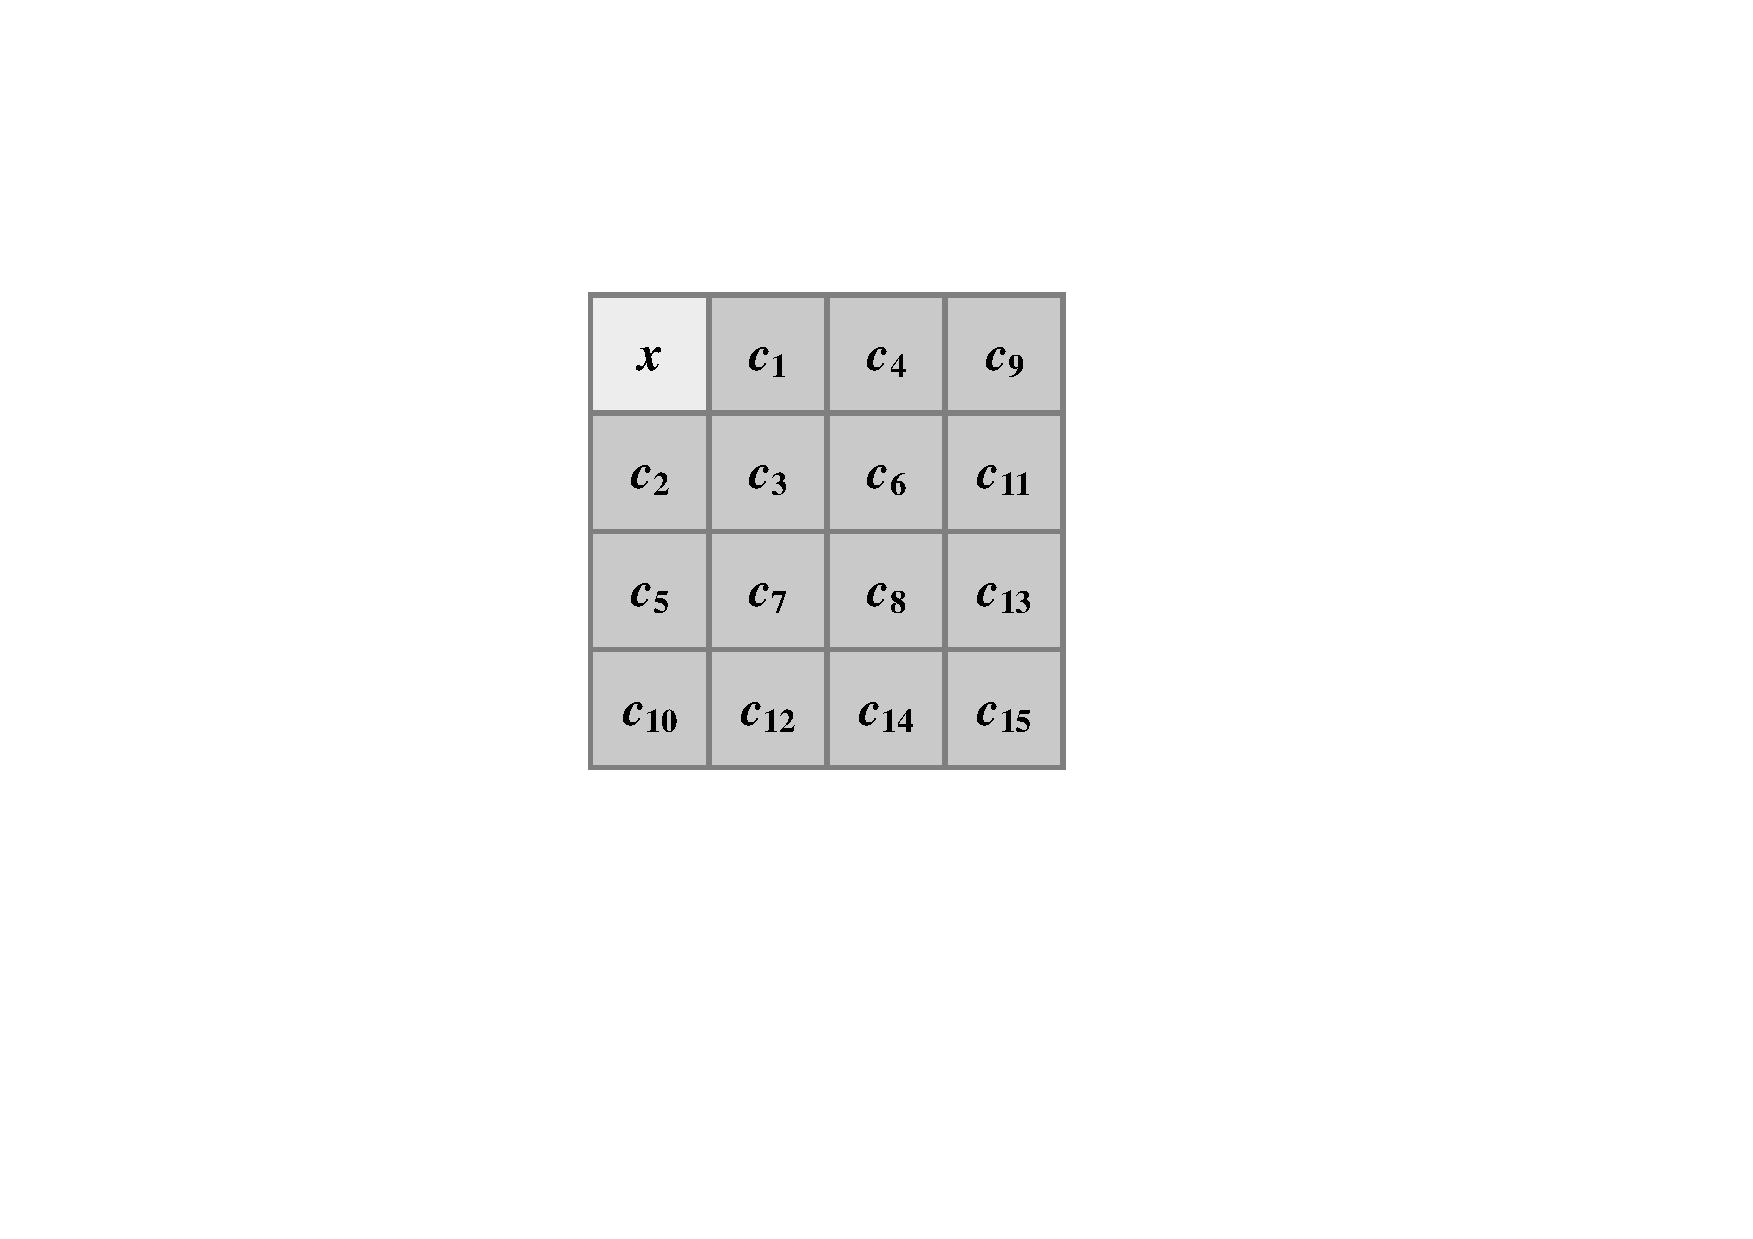
\includegraphics[width=1\textwidth]{figures/PPVOContext.pdf}
    \end{minipage}
}
\qquad\qquad
\subfigure[PEH with PPVO predictor on image Lena.]{
    \begin{minipage}[t]{0.42\linewidth}
    \centering
    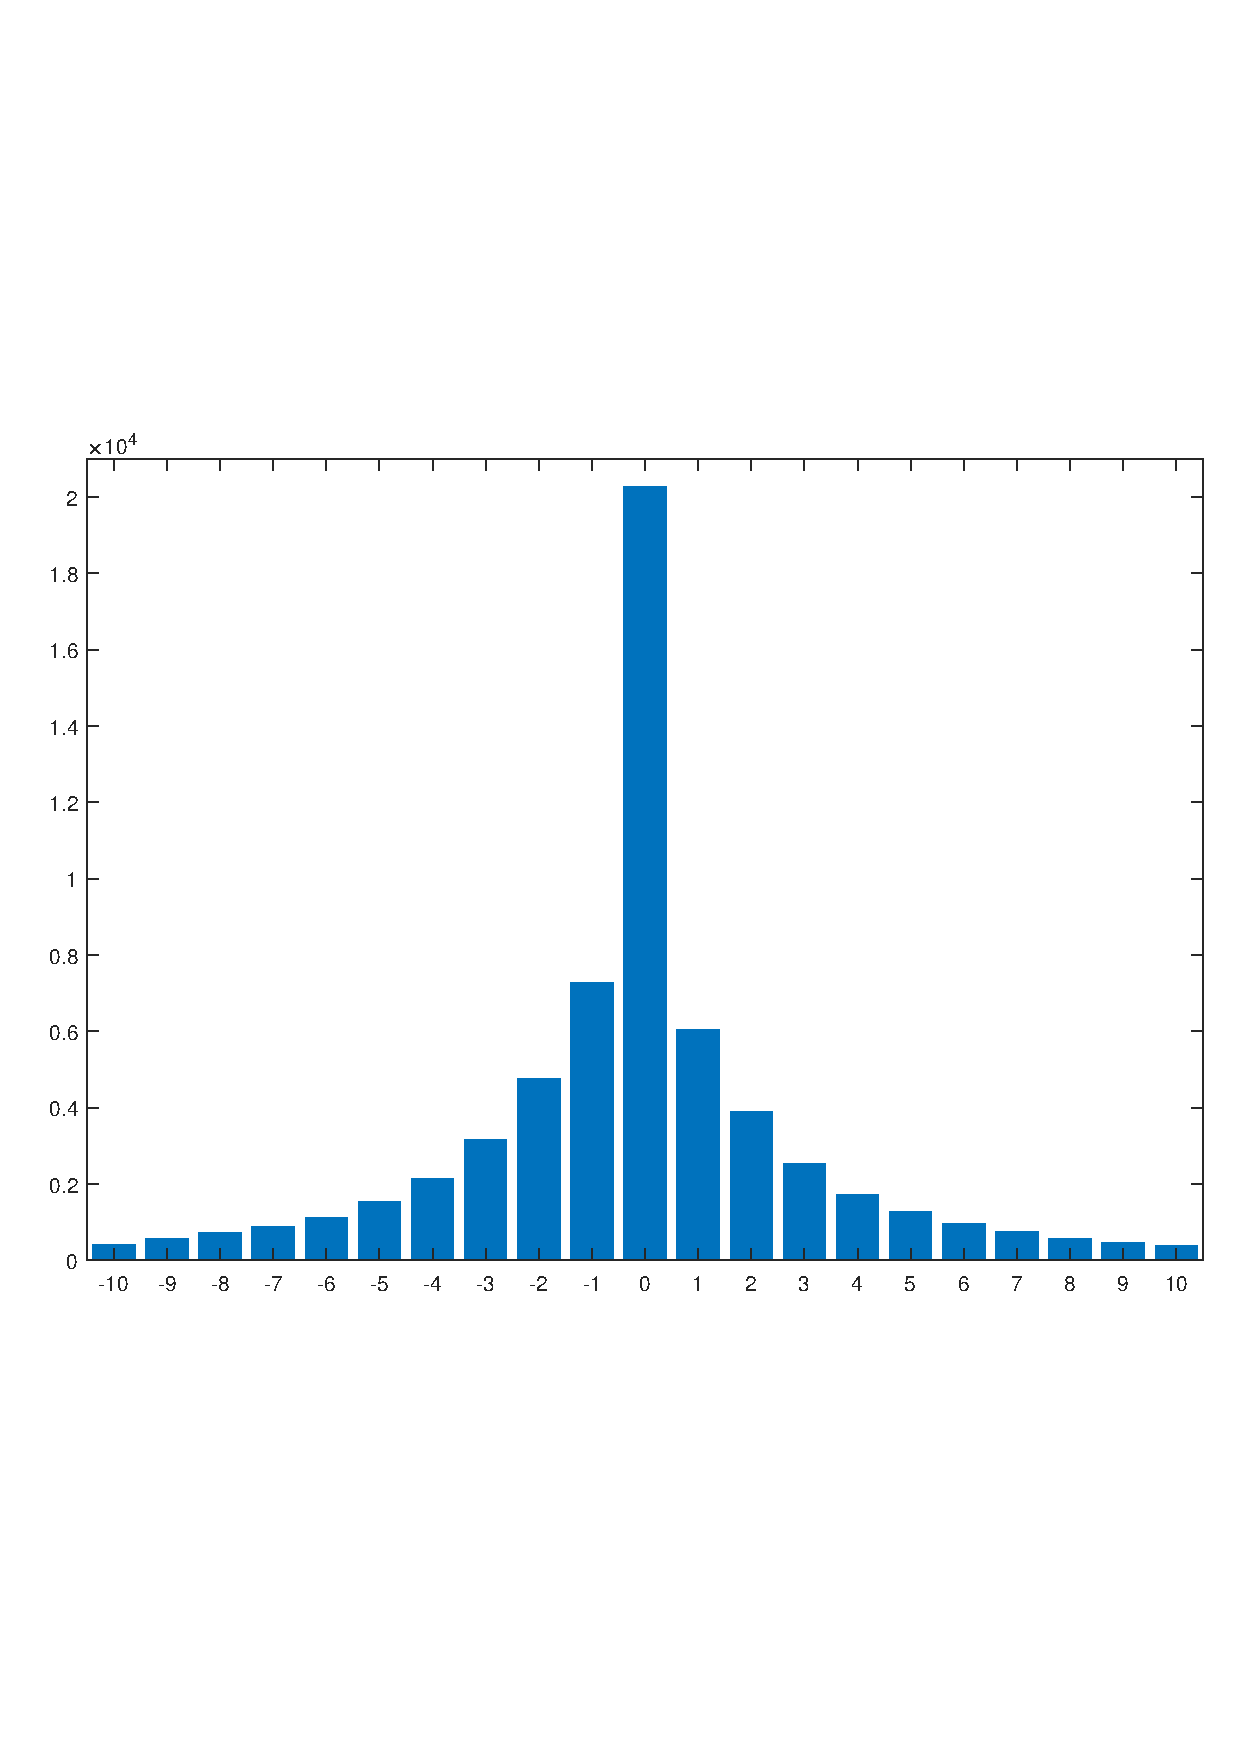
\includegraphics[width=1\textwidth]{figures/PPVO_Lena_CN15_hist_PN.pdf}
    \end{minipage}
}		
\centering
\caption{PPVO Context Pixels and show the shaper histogram with $n = 15$.}
\label{Fig.PPVOCNandHist}
\end{figure*}
Next, based on the sorted context pixels, four cases may occur in the process of the prediction of $x$. And pixels used for data embedding are accordingly grouped into four sets. They are
\begin{equation}\label{eq:S}
\begin{array}{ll}
    S_1 = \{ x | C_{\rm max} \neq C_{\rm min}, x \geq C_{\rm max} \} \\
    S_2 = \{ x | C_{\rm max} \neq C_{\rm min}, x \leq C_{\rm min} \} \\
    S_3 = \{ x | C_{\rm max}   =  C_{\rm min}, x \leq C_{\rm min}, C_{\rm min} \neq 254 \} \\
    S_4 = \{ x | C_{\rm max}   =  C_{\rm min}, x \geq C_{\rm max}, C_{\rm max} =  254 \} \\
\end{array}
\end{equation}
where $C_{\rm max}$ and $C_{\rm min}$ represent the largest and the smallest context pixels in $C$, respectively. Note that, other pixels which is not belong to these four sets are skipped and not utilized for embedding. In this way, $x$ can be predicted as $\hat{x}$ by
%\begin{itemize}
%  \item if $x$ belongs to $S_1$ or $S_4$, $\hat{x} = C_{\rm max}$,
%  \item if $x$ belongs to $S_2$ or $S_3$, $\hat{x} = C_{\rm min}$.
%\end{itemize}
\begin{equation}\label{eq:xhat1}
    \hat{x} = \left\{\begin{array}{ll}
    C_{\rm max},  & \text{if } x \in S_1 \bigcup S_4 \\
    C_{\rm min},  & \text{if } x \in S_2 \bigcup S_3 
\end{array}\right.
.
\end{equation}
And the prediction-error $e$ is computed by
\begin{equation}\label{eq:PE}
e = x - \hat{x}.
\end{equation}
Here, the standard $512 \times 512$ sized gray-scale image Lena is taken for example, and the PEH is shown in Fig. \ref{Fig.PPVOCNandHist}(b), in which the highest frequency locates at bin 0. Therefore, bin 0 is used for expansion, and other bins are shifted to create vacancies. That is to say, the prediction-error $e$ is modified to $\tilde{e}$ to embed data as
\begin{equation}\label{eq:PPVOMPE}
    \tilde{e} = \left\{\begin{array}{ll}
    e + b,  & \text{if } e = 0, x \in S_1 \cup S_4 \\
    e - b,  & \text{if } e = 0, x \in S_2 \cup S_3 \\
    e + 1,  & \text{if } e \geq 1 \\
    e - 1,  & \text{if } e \leq -1
\end{array}\right.
\end{equation}
where $b \in \{0,1\}$ is a data bit to be embedded. Accordingly, the marked pixel $\tilde{x}$ is determined as
\begin{equation}\label{eq:PPVOMPixel}
    \tilde{x} = \hat{x} + \tilde{e}.
\end{equation}

Notice that, the embedding process for a cover image is performed in the raster-scan order and the extraction process is implemented in reverse order. Thus, the context pixels of a cover pixel and its corresponding marked pixel are the same. Due to the fact that, in the embedding process, for $x \in S_1 \cup S_4$, it is either increased by 1 or unchanged, and for $x \in S_2 \cup S_3$, it is either decreased by 1 or unchanged, the marked pixel $\tilde{x}$ can be classified into the same group with $x$ according to \eqref{eq:S}.
Therefore, to extract the data bit and recover the original cover pixel, the prediction of the marked pixel $\tilde{x}$ is conducted in the same way as embedding process. First,
\begin{equation}\label{eq:xhat2}
    \hat{x} = \left\{\begin{array}{ll}
    C_{\rm max},  & \text{if } \tilde{x} \in S_1 \bigcup S_4 \\
    C_{\rm min},  & \text{if } \tilde{x} \in S_2 \bigcup S_3
\end{array}\right.
.
\end{equation}
Then, the marked prediction-error $\tilde{e}$ is computed by
\begin{equation}\label{eq:dPE}
\tilde{e} = \tilde{x} - \hat{x},
\end{equation}
Next, it is modified to obtain the prediction-error $e$ by
\begin{equation}\label{eq:dPPVOMPE}
e = \left\{\begin{array}{ll}
\tilde{e},      & \text{if } e = 0      \\
\tilde{e} - 1,  & \text{if } e \geq 1   \\
\tilde{e} + 1,  & \text{if } e \leq -1
\end{array}\right..
\end{equation}
Finally, the original cover pixel $x$ is recovered by
\begin{equation}\label{eq:dPPVOX}
x = \hat{x} + e.
\end{equation}
Meanwhile, the secret data bit is extracted as $b = 1$ if $\tilde{e} \in \{-1, 1\}$ and $b = 0$ if $\tilde{e} = 0$.

Besides, in the embedding process, the proper number of context pixels is exhaustively determined by setting $n$ from 1 to 15 for embedding, and the one generating marked image with highest PSNR will be selected. In addition, to better exploit the image redundancy, a pixel selection strategy with a threshold $T$ is employed to improve the embedding performance. And, pixels whose local complexity is smaller than $T$ will be used for embedding. In detail, the complexity of each pixel is defined as the difference of the maximum and the minimum of its 15 context pixels, as illstated in Fig. \ref{Fig.PPVOCNandHist}(a). Experimental results show that this method provides larger embedding capacity than the previous PVO-based methods \cite{Li2013PVO,Peng2014IPVO} due to the use of pixel-by-pixel prediction. At the same time, sharper histograms which contribute to the better embedding performance are obtained by this method.

Actually, the PPVO method can be improved from two aspects. On one hand, since the context pixels of $x$ are chosen from the down right direction of the target pixel, other pixels in the down left direction, which is more close to $x$ and more useful for accurate prediction, are not fully exploited. On the other hand, in PPVO, pixels are predicted with a fixed number of context pixels. However, various context pixels number $n$ on pixels of different local complexity have different effects. Therefore, to better exploit the context pixels as well as the difference of pixel local complexity, we proposed an improved PPVO method, and the details will be introduced in the next section.
 



%----------------------------------------------------------------------------------------
\section{Proposed Method}\label{sec:3}
In this section, a extended PPVO predictor is first introduced. Then, a multi-size based embedding method for MHM is proposed to further improve the performance. Finally, the embedding procedure and extraction procedure is described.

\subsection{Extended PPVO predictor}\label{sec:3.1}
Compared with PVO-based methods such as PVO\cite{Li2013PVO}, IPVO\cite{Peng2014IPVO} and PVO-\emph{k}\cite{Ou2014PVOk}, in PPVO, every pixel is predicted for embedding, breaking through the block constraint. And to ensure the reversibility, pixels in lower right direction are utilized as context region to predict the current pixel which is shown in Fig. \ref{Fig.Context}(a) and Fig. \ref{Fig.Context}(c). The prediction is more accurate, however, the surrounding context information is not fully utilized. There are some other pixels are omitted. Clearly, for example, pixels $\{C_4\}$ in Fig. \ref{Fig.Context}(b) and $\{c_{4}, c_{7}, c_{8}\}$ in Fig. \ref{Fig.Context}(d) are closer to current pixel $x$ and can provide more useful information, but they are omitted in pixel prediction stage. The extended PPVO predictor introduces this information and the superiority of extended PPVO predictor is introduced next.
\begin{figure*}
\centering
\subfigure[PPVO predictor with $n=4$]{
    \begin{minipage}[t]{0.2\linewidth}
    \centering
    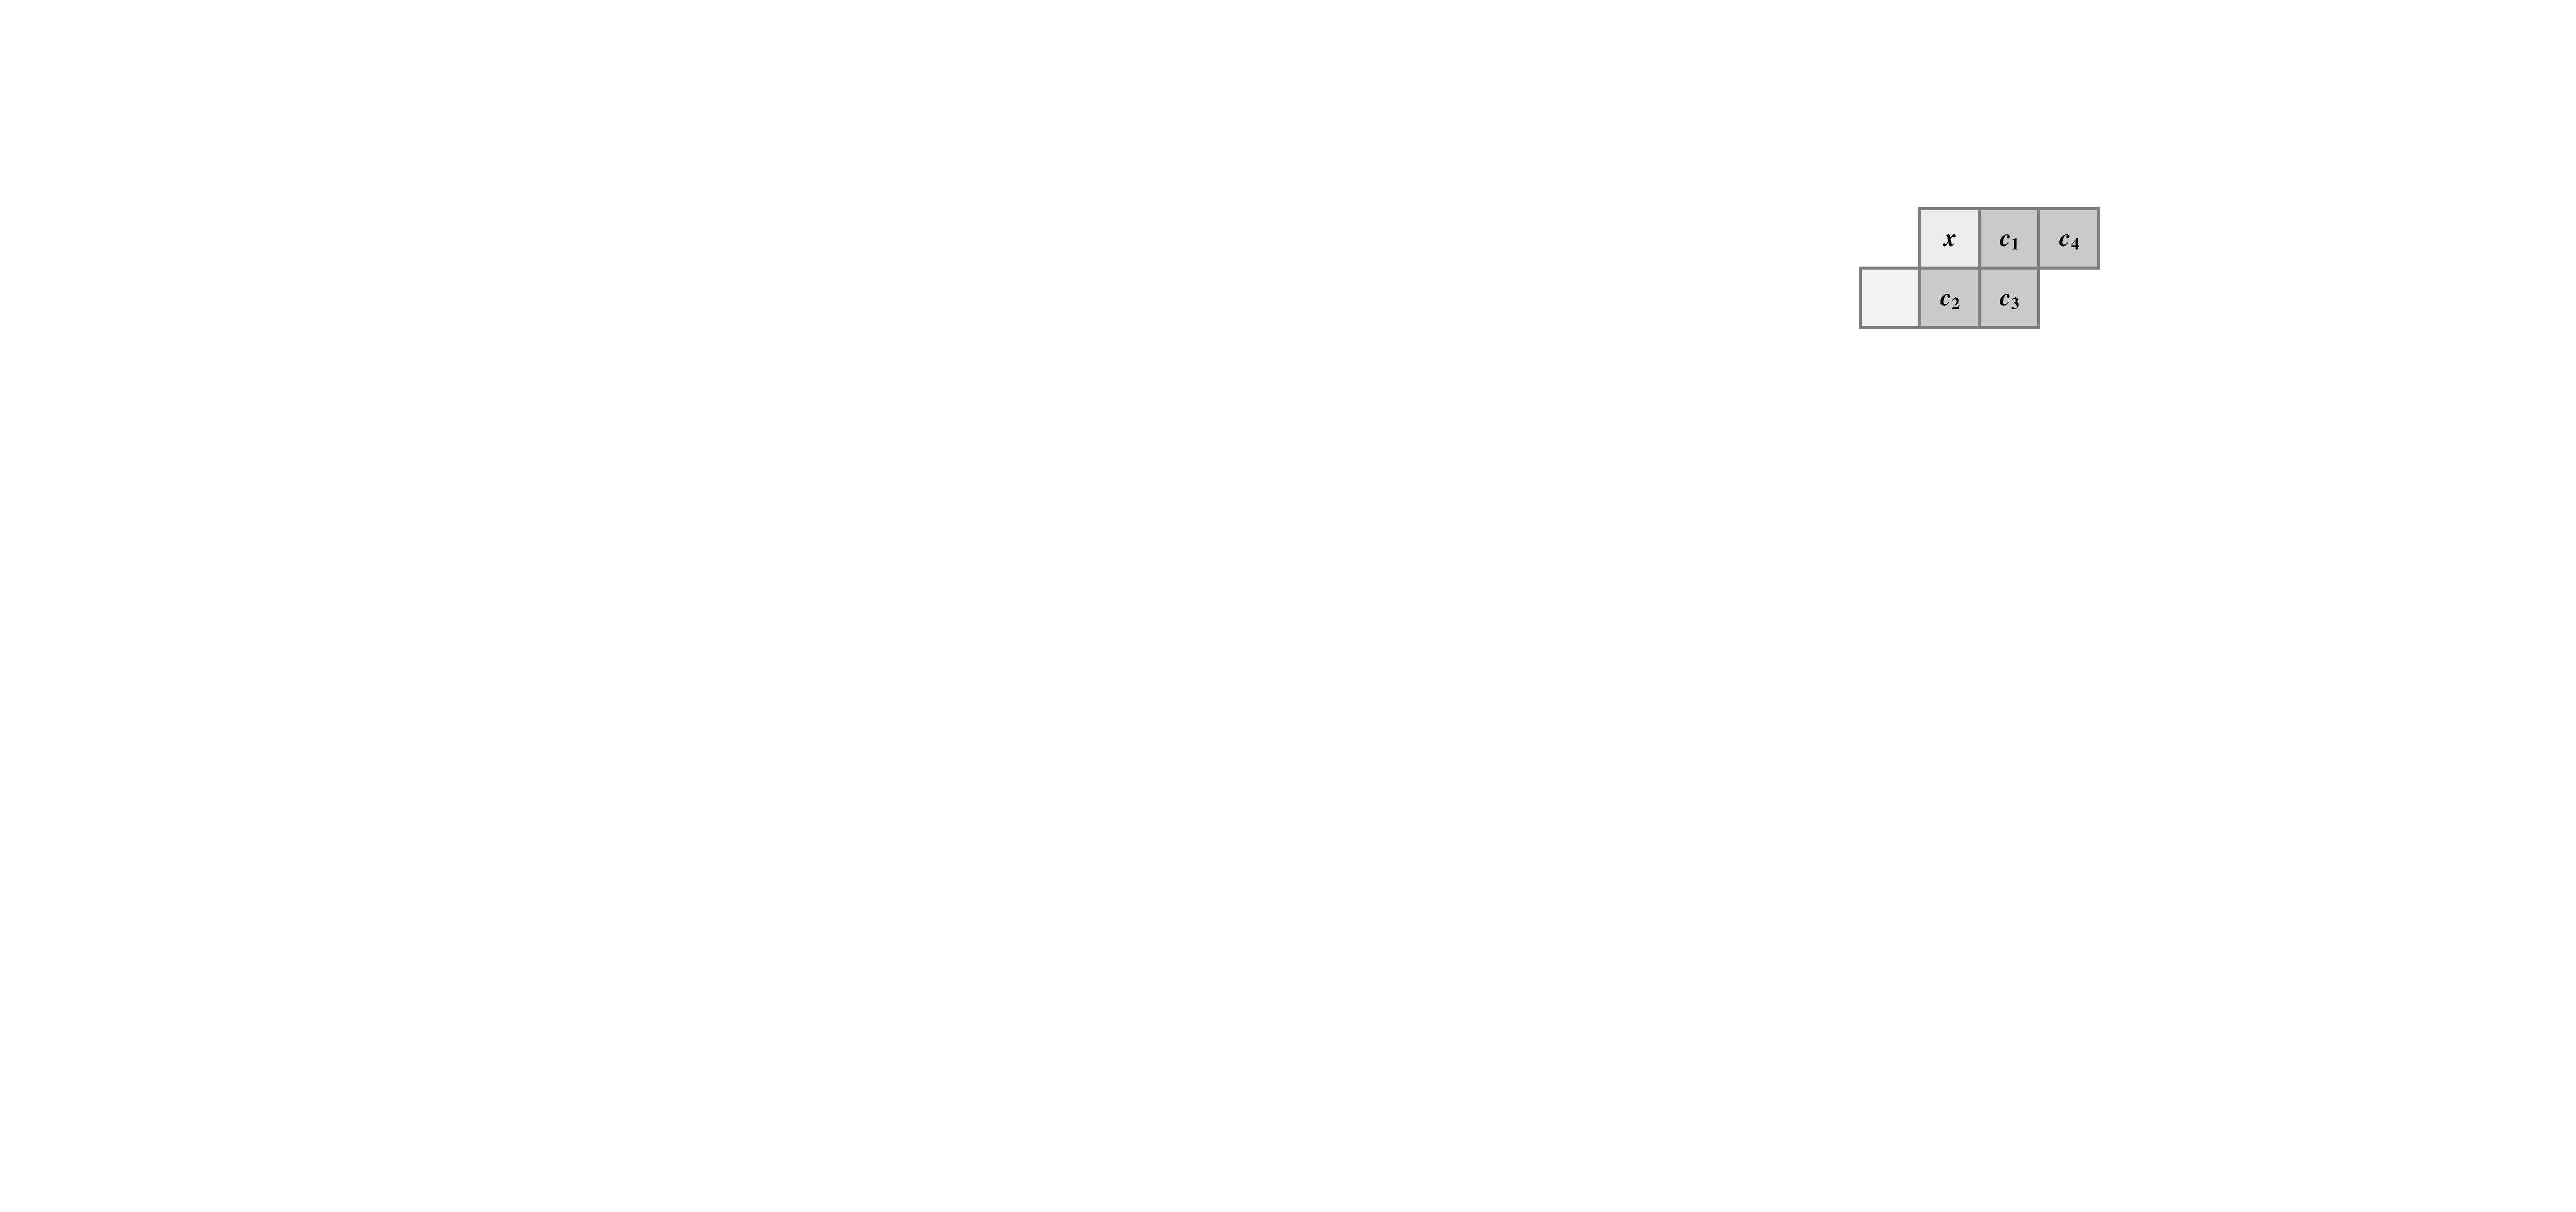
\includegraphics[width=1\textwidth]{figures/CN4a.pdf}
    \end{minipage}
}
\qquad\qquad
\subfigure[Extended PPVO predictor with $n=8$.]{
    \begin{minipage}[t]{0.2\linewidth}
    \centering
    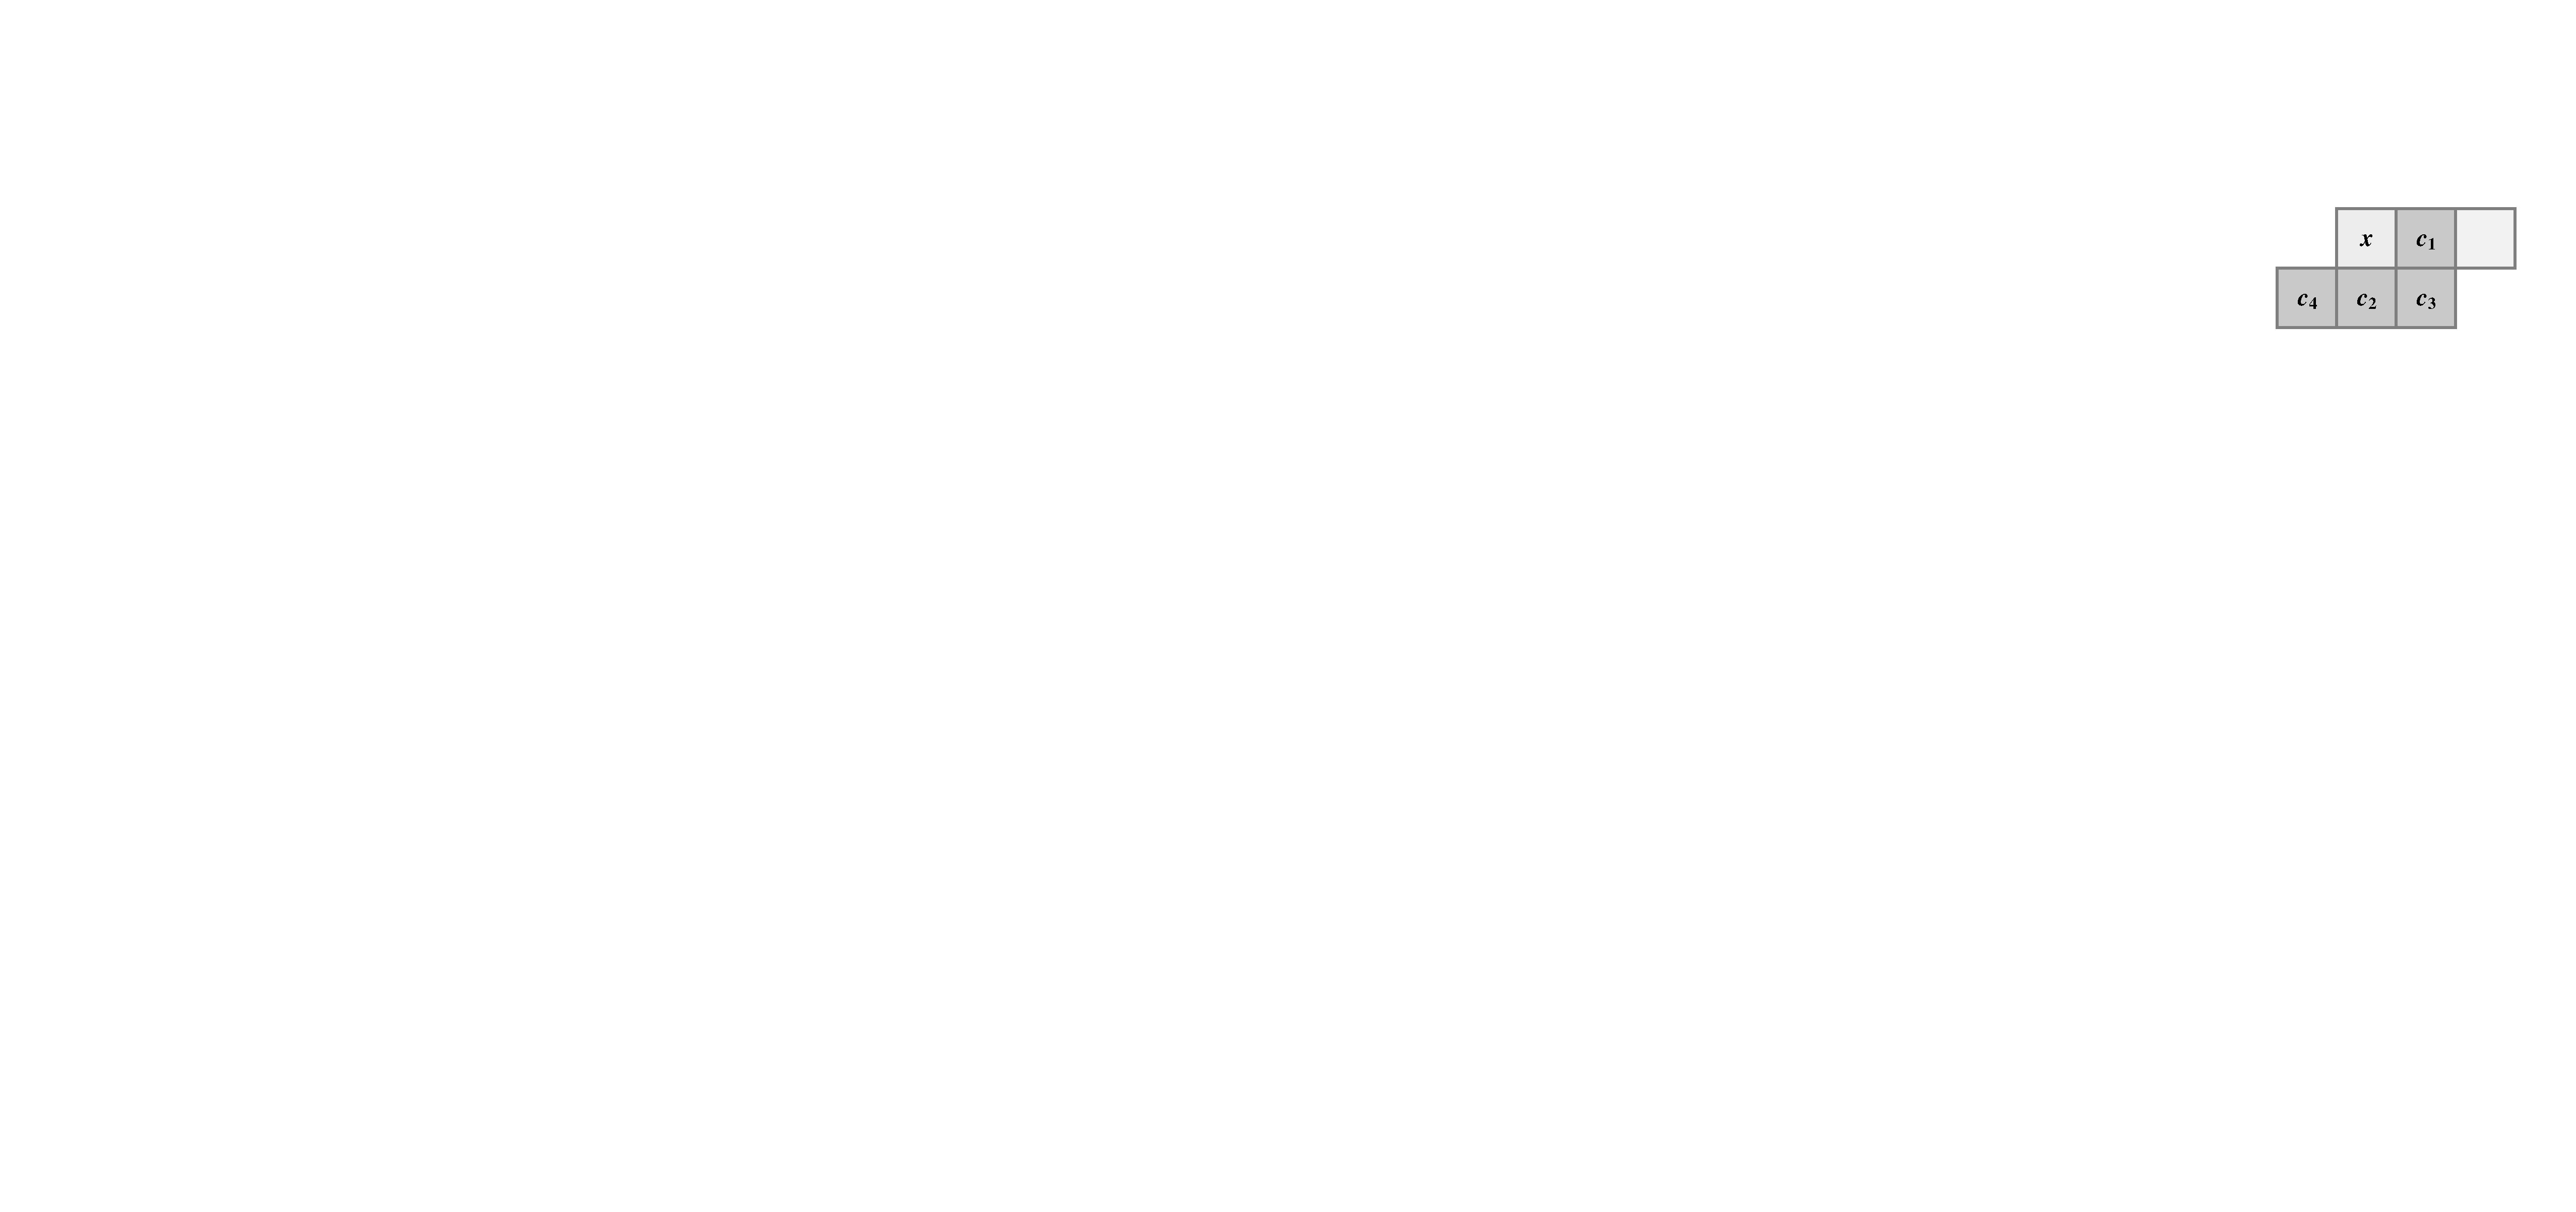
\includegraphics[width=1\textwidth]{figures/CN4b.pdf}
    \end{minipage}
}

\subfigure[PPVO predictor with $n=8$]{
    \begin{minipage}[t]{0.2\linewidth}
    \centering
    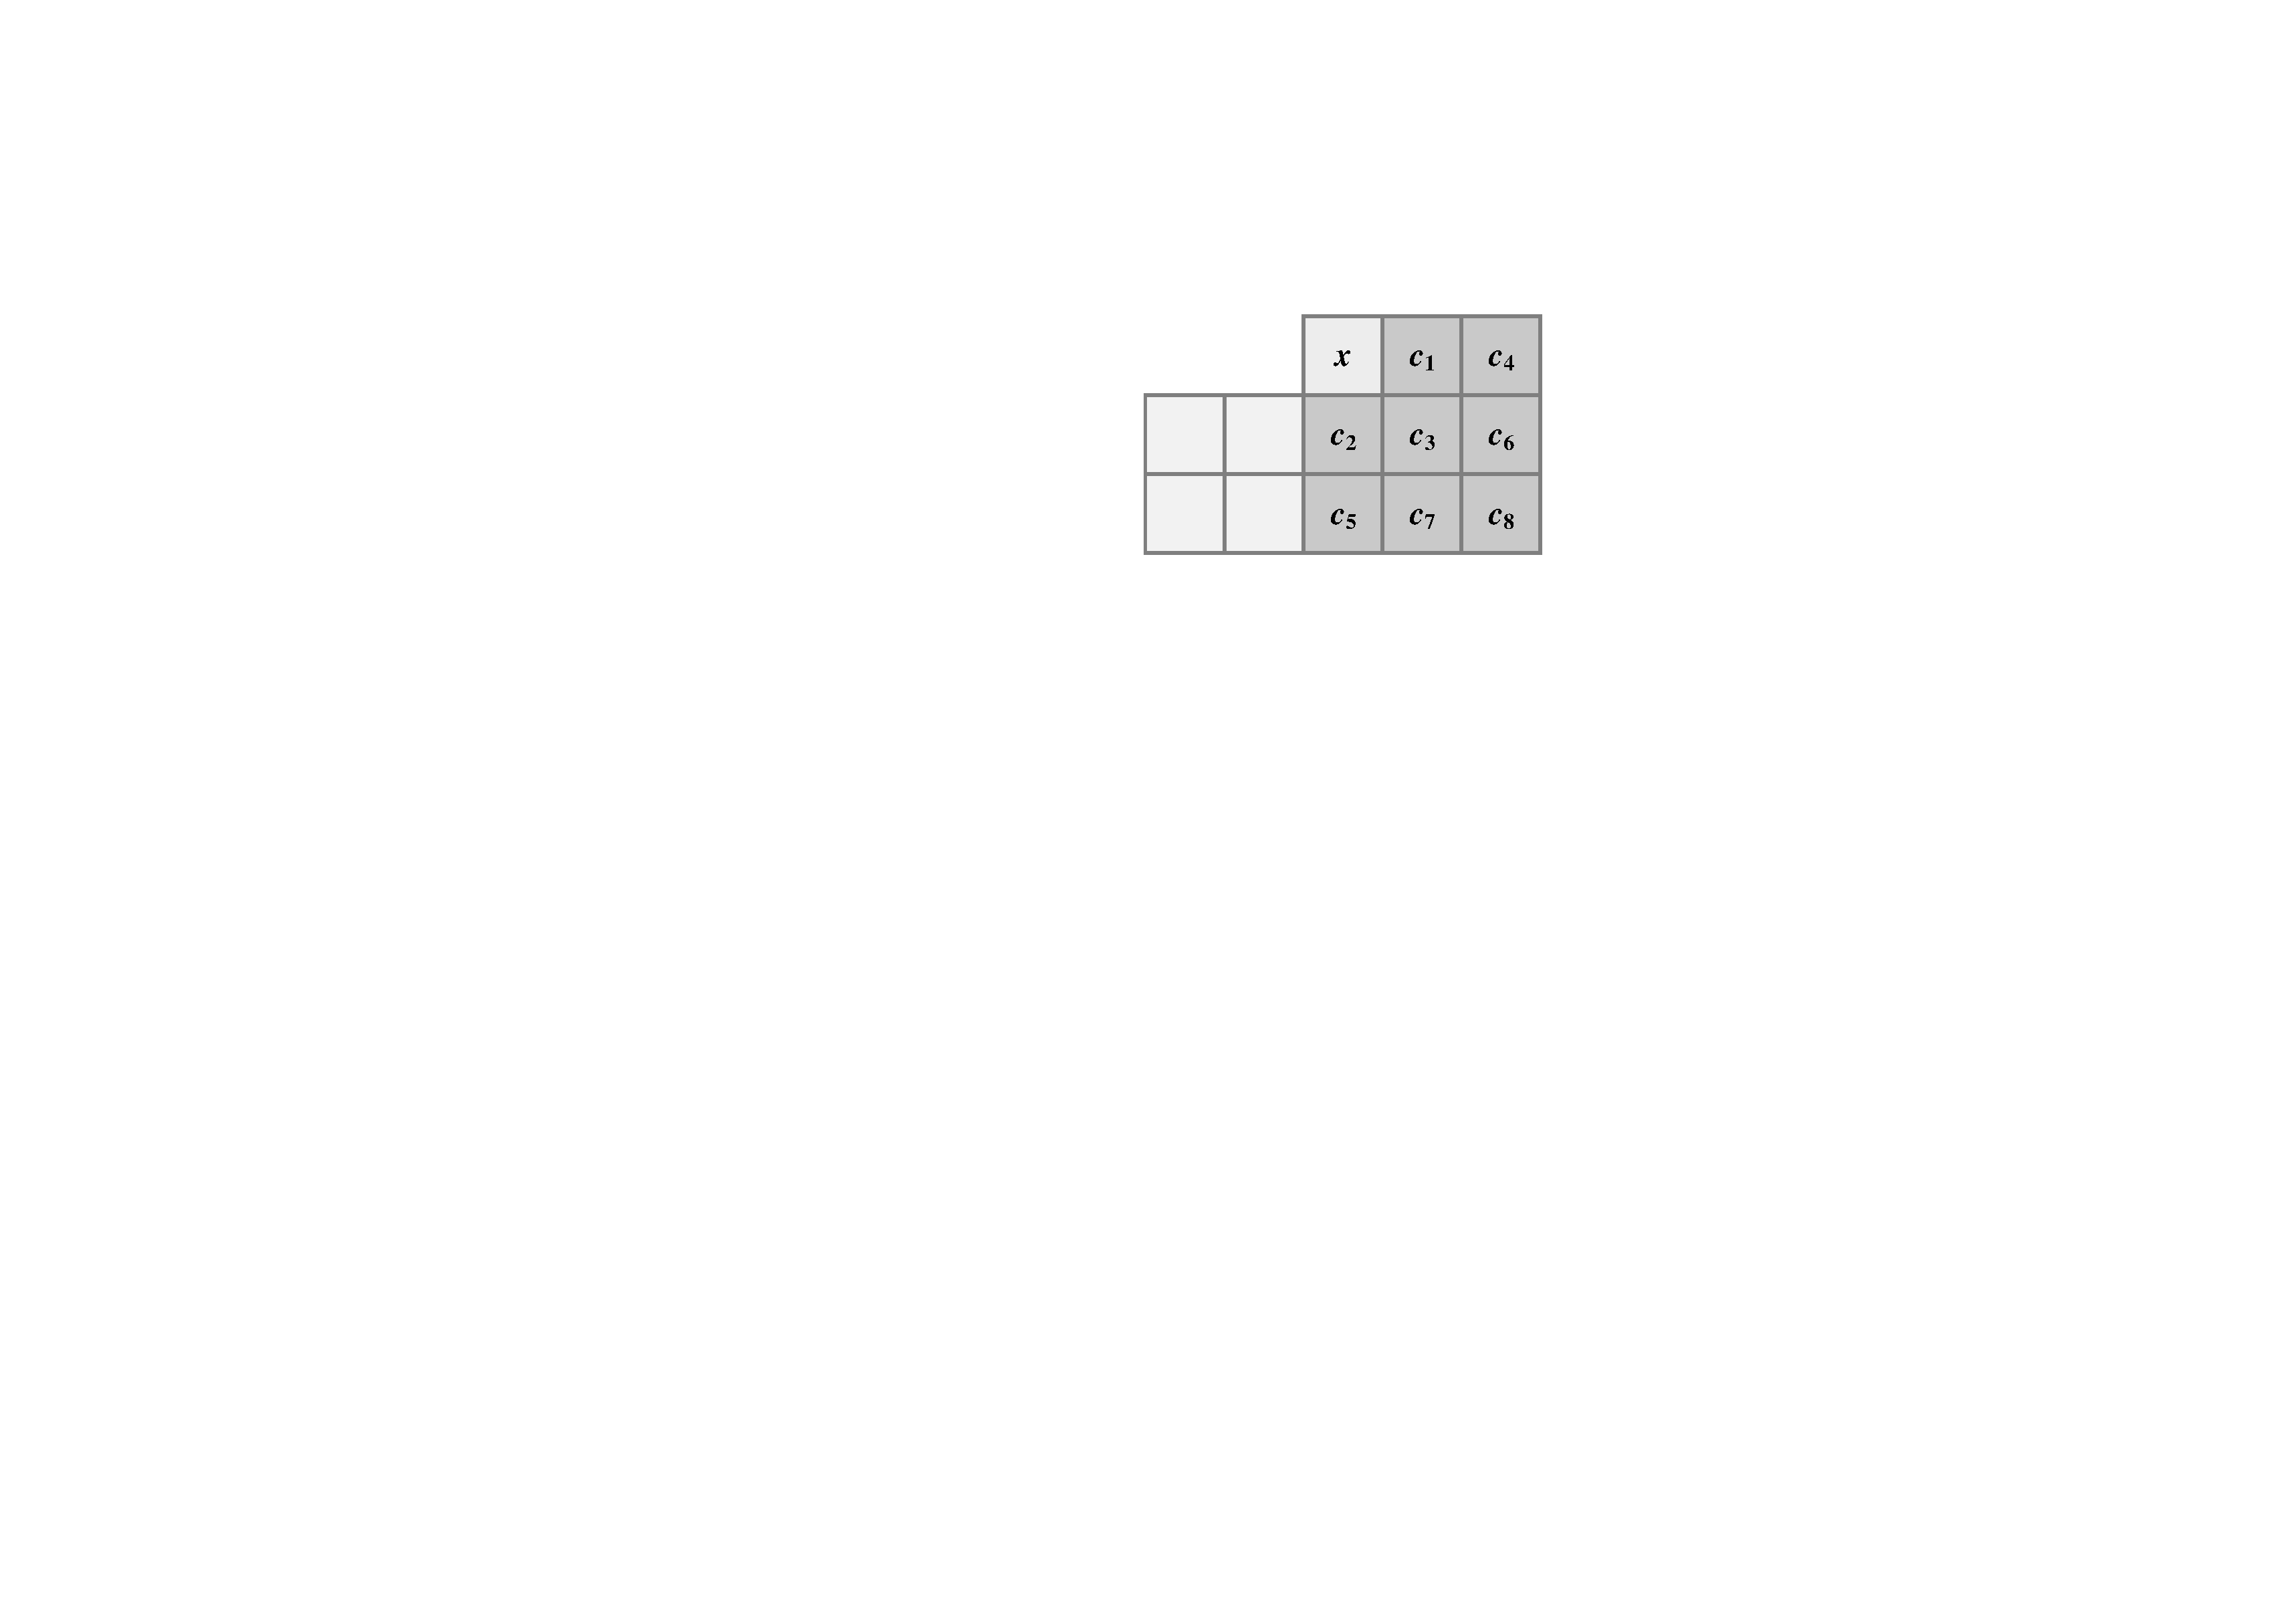
\includegraphics[width=1\textwidth]{figures/CN8a.pdf}
    \end{minipage}
}
\qquad\qquad
\subfigure[Extended PPVO predictor with $n=8$.]{
    \begin{minipage}[t]{0.2\linewidth}
    \centering
    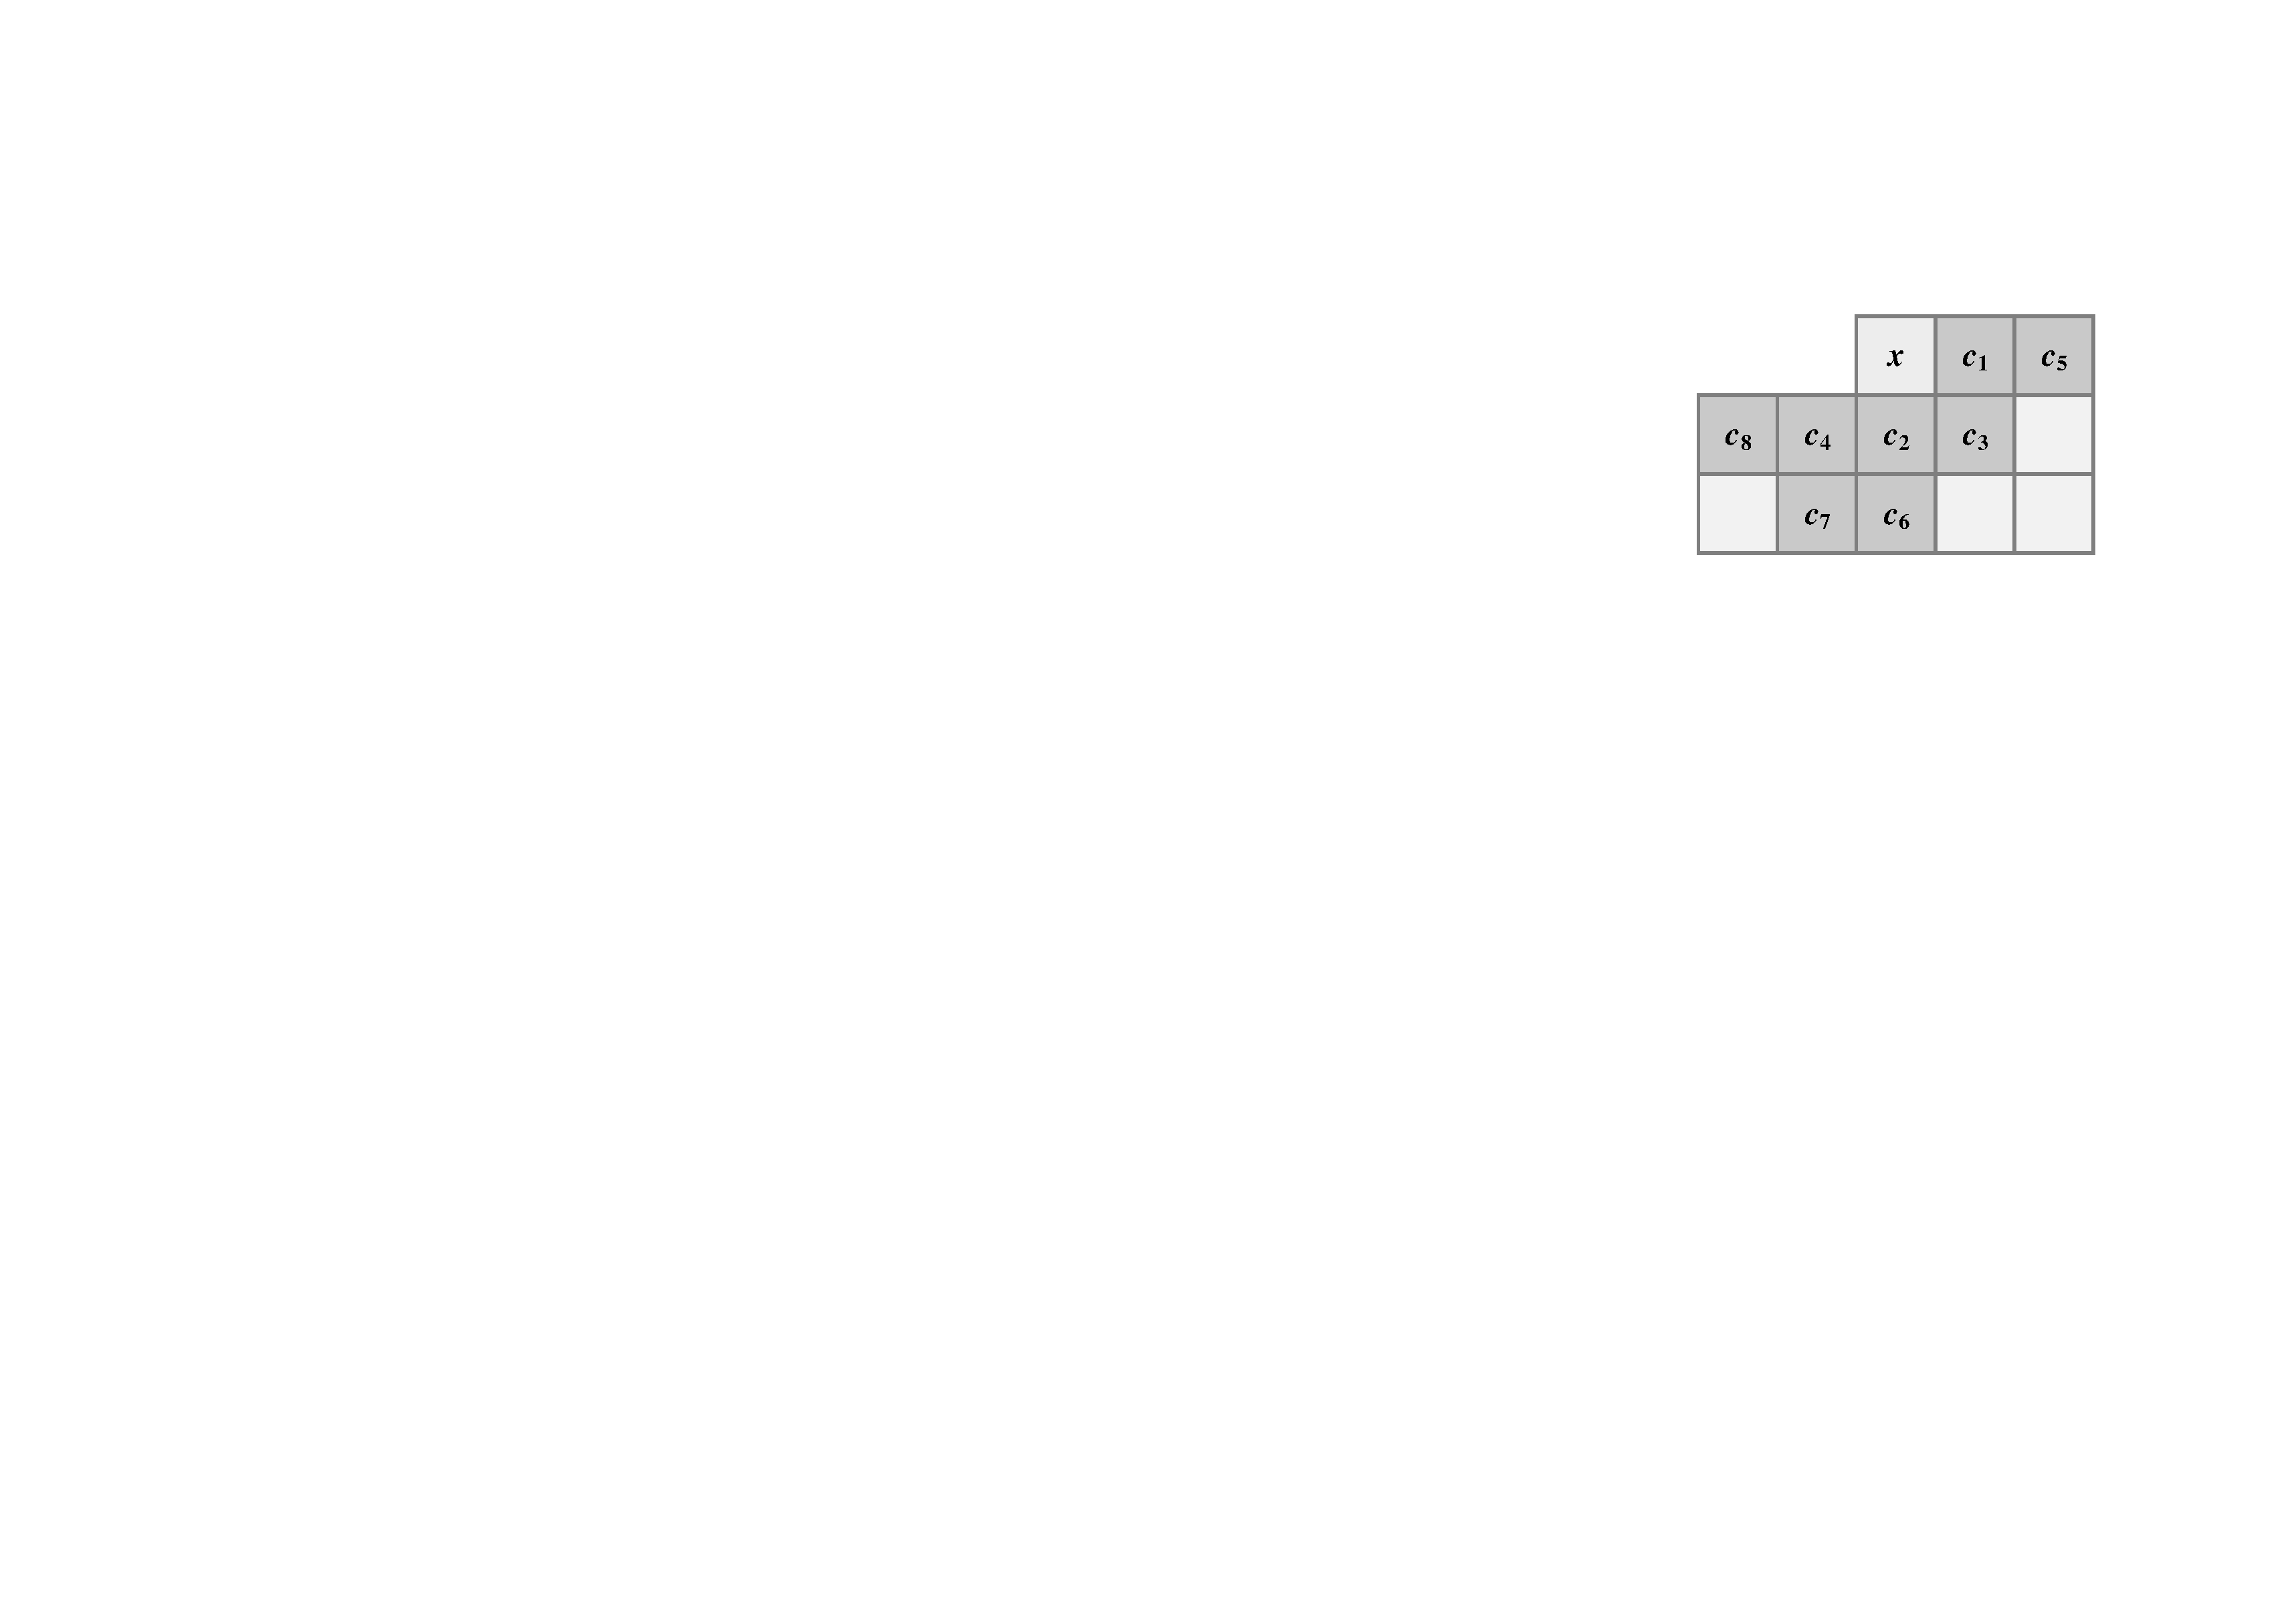
\includegraphics[width=1\textwidth]{figures/CN8b.pdf}
    \end{minipage}
}		
\centering
\caption{Context pixels of $x$ by extended PPVO predictor.}
\label{Fig.Context}
\end{figure*}

Fig. \ref{Fig.ComparisonEPPVO} shows the comparison of normalized PEHs of extended PPVO predictor and original PPVO predictor are displayed on two standard gray-scale $512 \times 512$ sized images with $n = 4$ and $n = 8$, respectively. For a reasonable comparison, in Fig. \ref{Fig.ComparisonEPPVO}(a) and Fig. \ref{Fig.ComparisonEPPVO}(b), four pixels near $x$ is considered as the context pixels. Fig. \ref{Fig.Context}(a) and Fig. \ref{Fig.Context}(b) show the context pixels selection for the PPVO predictor and the extended PPVO predictor. And in Fig. \ref{Fig.ComparisonEPPVO}(c) and Fig. \ref{Fig.ComparisonEPPVO}(d), Fig. \ref{Fig.Context}(c) and Fig. \ref{Fig.Context}(d) show the eight context pixels selection for the PPVO predictor and the extended PPVO predictor.

Obviously, normalized PEHs of extended PPVO predictor have highest peak at $0$, and the distributions are sharper, which is beneficial to the final embedding performance.
Moreover, we use the proportion of shifted pixels \cite{Li2013PVO} to evaluate characteristic of the histogram theoretically, numerically expressed as
\begin{equation}\label{eq:Pshift}
    \frac{\#\{{\rm shifted\ pixels}\}}{\#\{{\rm expanded\ or\ shifted\ pixels}\}} = \frac{\sum_{i \neq 0}{\rm H}(i)}{{\rm H}(0) + \sum_{i \neq 0}{\rm H}(i)},
\end{equation}
where ${\rm H}$ is the PEH and ${\rm H}(i)$ is the frequency of pixels whose prediction-errors $p = i$. This evaluation describes the distortion caused by embedding one bit data on ${\rm H}$. The smaller the proportion of shifted pixels, the better the characteristics of the PEH, which can bring less distortion. In Fig. \ref{Fig.ComparisonEPPVO}, for images Lena, and Baboon, with $n = 4$, proportion of of extended PPVO predictor are 0.65, and 0.88 respectively, while value of evaluation are 0.72, and 0.89 of PPVO predictor. This indicates that data embedding on PEH of extended PPVO predictor may carry much less distortion to obtain the better performance. And with $n = 8$, proportion of of extended PPVO predictor are 0.61, and 0.86 respectively, while value of evaluation are 0.7, and 0.88 of PPVO predictor. This indicates that data embedding on PEH of extended PPVO predictor may carry much less distortion to obtain the better performance.
\begin{figure*}
\centering
\subfigure[Lena, $n = 4$]{
    \begin{minipage}[t]{0.4\linewidth}
    \centering
    \includegraphics[width=1\textwidth]{figures/Comparison/4Pixels/lena1.pdf}
    \end{minipage}
}
\qquad
\subfigure[Baboon, $n = 4$]{
    \begin{minipage}[t]{0.4\linewidth}
    \centering
    \includegraphics[width=1\textwidth]{figures/Comparison/4Pixels/baboon1.pdf}
    \end{minipage}
}


\subfigure[Lena, $n = 8$]{
    \begin{minipage}[t]{0.4\linewidth}
    \centering
    \includegraphics[width=1\textwidth]{figures/Comparison/8Pixels/lena1.pdf}
    \end{minipage}
}
\qquad
\subfigure[Baboon, $n = 8$]{
    \begin{minipage}[t]{0.4\linewidth}
    \centering
    \includegraphics[width=1\textwidth]{figures/Comparison/8Pixels/baboon1.pdf}
    \end{minipage}
}
\centering
\caption{Comparison of normalized PEH of $p$ of extended PPVO with context pixels in Fig. \ref{Fig.Context}.}
\label{Fig.ComparisonEPPVO}
\end{figure*}


\subsection{Multi-size based Embedding Method for MHM}\label{sec:3.2}
In PPVO, before implementing the embedding procedure, number of context pixels $n$ of to-be-predicted $x$ is already set in advance. And for a cover image, every pixel is predicted by the same region of context pixels. Actually, the performance results caused by different number of context pixels are different. In order to explore the impact of $n$, we consider $n \leq 24$ and, to simplify the presentations, context pixels are group into four sets according to size of the region around the current pixel $x$, including $C_1 = \{c_1, ..., c_4\}$, $C_2 = \{c_1, ..., c_{10}\}$, $C_3 = \{c_1, ..., c_{18}\}$ and $C_4 = \{c_1, ..., c_{24}\}$, as shown in Fig. \ref{Fig.Context3}. Based on the consideration of the complexity of traditional RDH embedding, the comparison of threshold-capacity curves and threshold-proportion curves are shown in Fig. \ref{Fig.Eval}(a) and Fig. \ref{Fig.Eval}(b) as well.
Here the proportion indicates the proportion of shifted pixels refined by (\ref{eq:Pshift}). And the threshold $T$ is set to choose the smooth pixels whose complexity ${\rm NL} < T$ to generate PEH so that all secret data can just be embedded. The complexity of the current pixel is evaluated by the sum of the absolution differences of the horizontal and vertical of every two adjacent pixels belong to the corresponding context. Besides, the capacity is defined as the occurrence of bin 0 of the generated PEH.

\begin{figure*}
\subfigure[$C_1$ of $n = 4$]{
    \begin{minipage}[t]{0.218\linewidth}
    \centering
    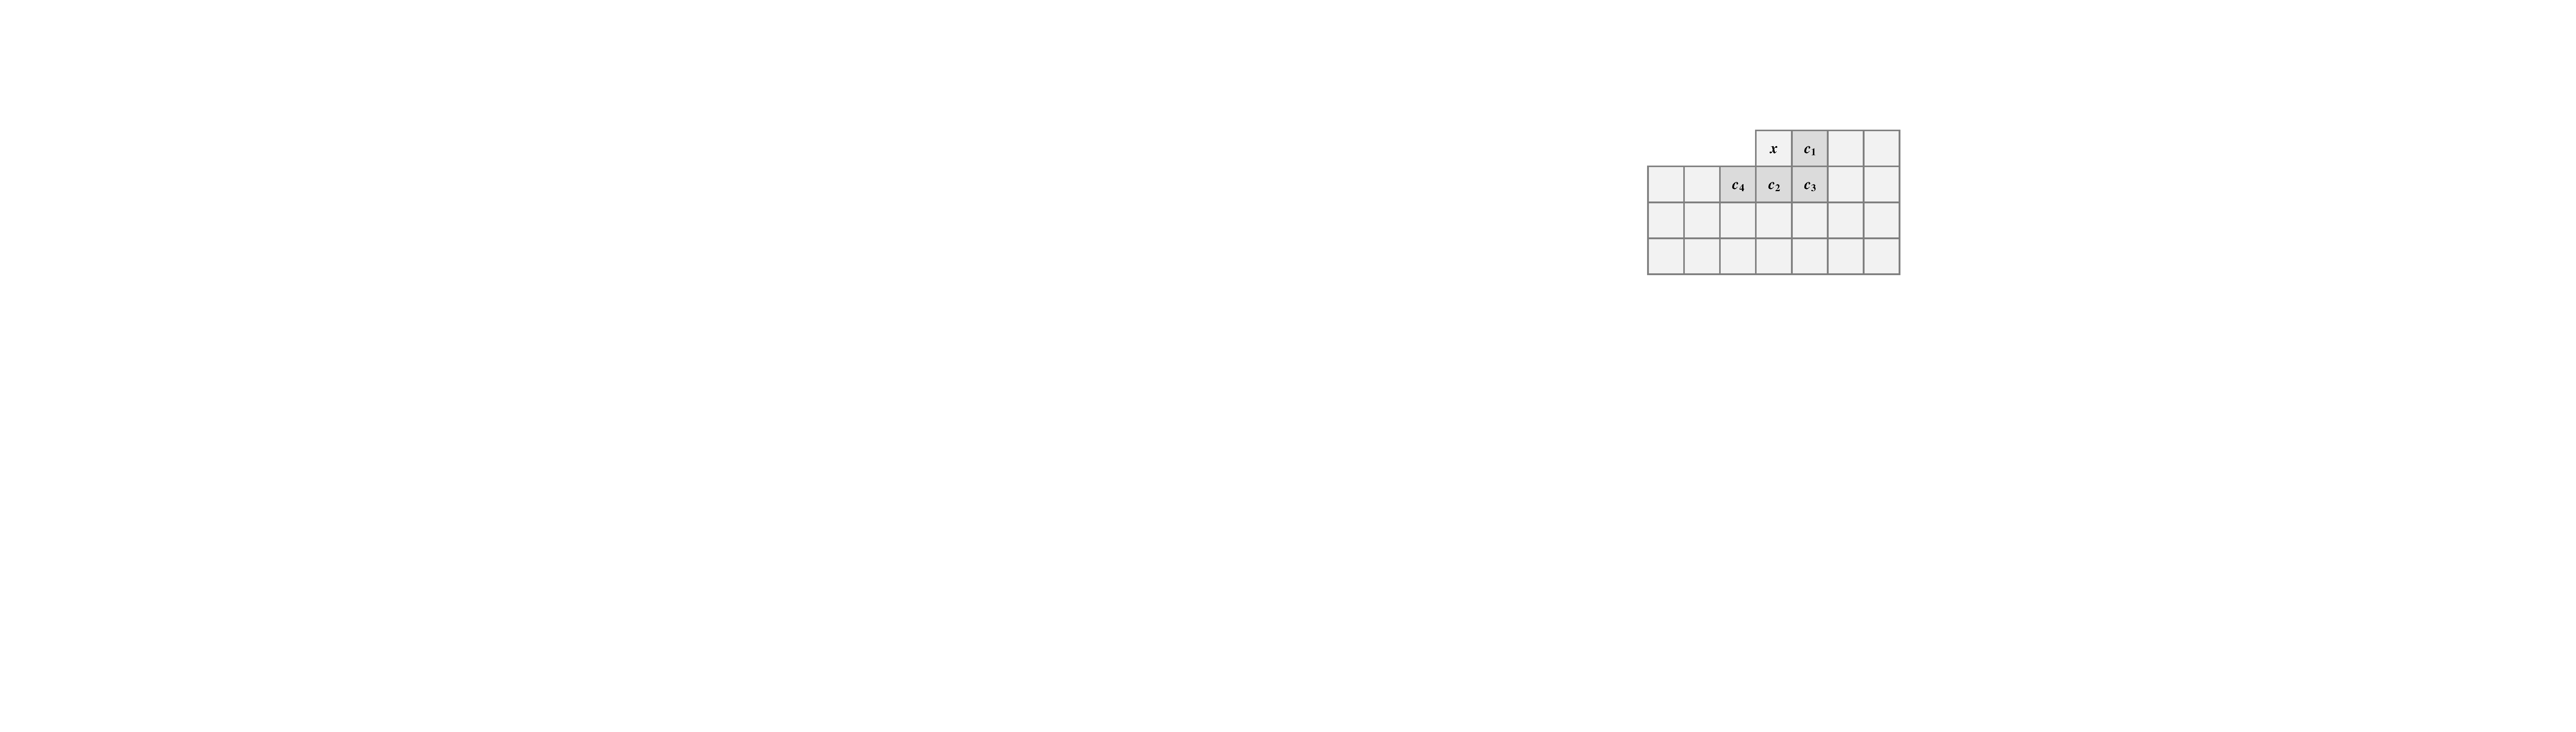
\includegraphics[width=1\textwidth]{figures/C1.pdf}
    \end{minipage}
}
\subfigure[$C_2$ of $n = 10$]{
    \begin{minipage}[t]{0.218\linewidth}
    \centering
    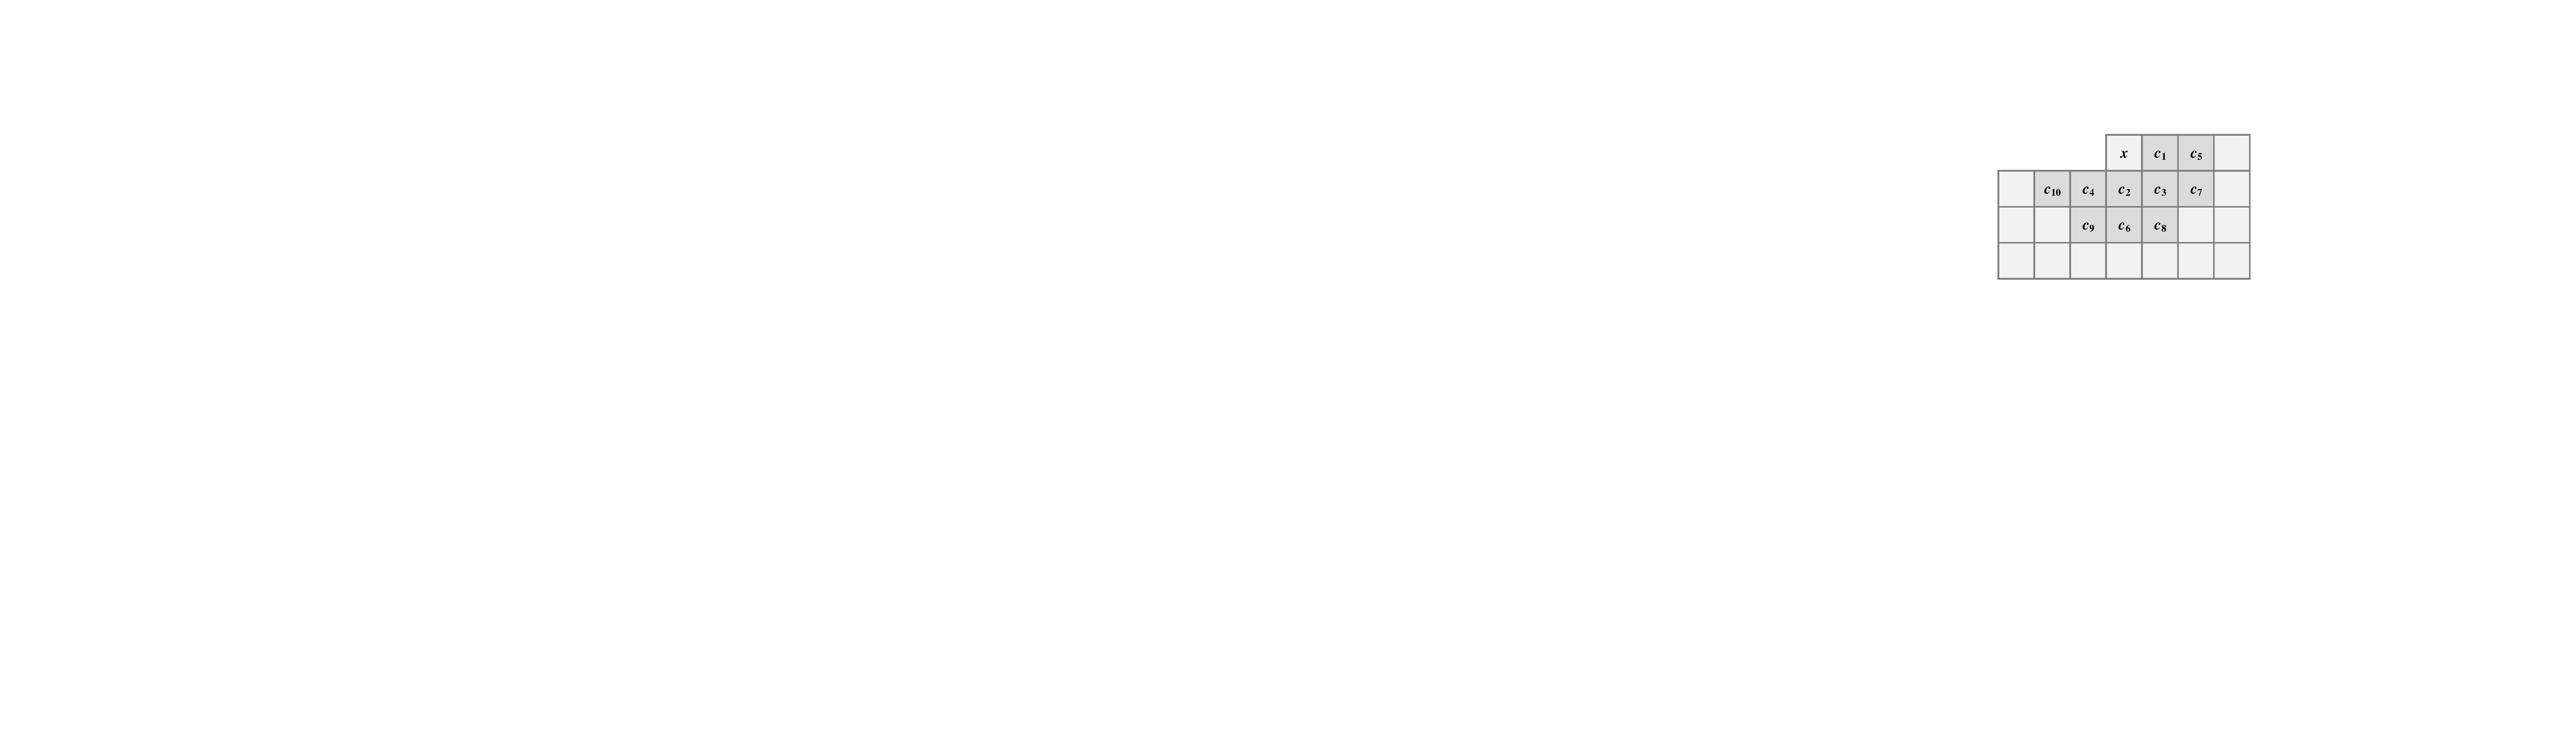
\includegraphics[width=1\textwidth]{figures/C2.pdf}
    \end{minipage}
}
\subfigure[$C_3$ of $n = 18$]{
    \begin{minipage}[t]{0.218\linewidth}
    \centering
    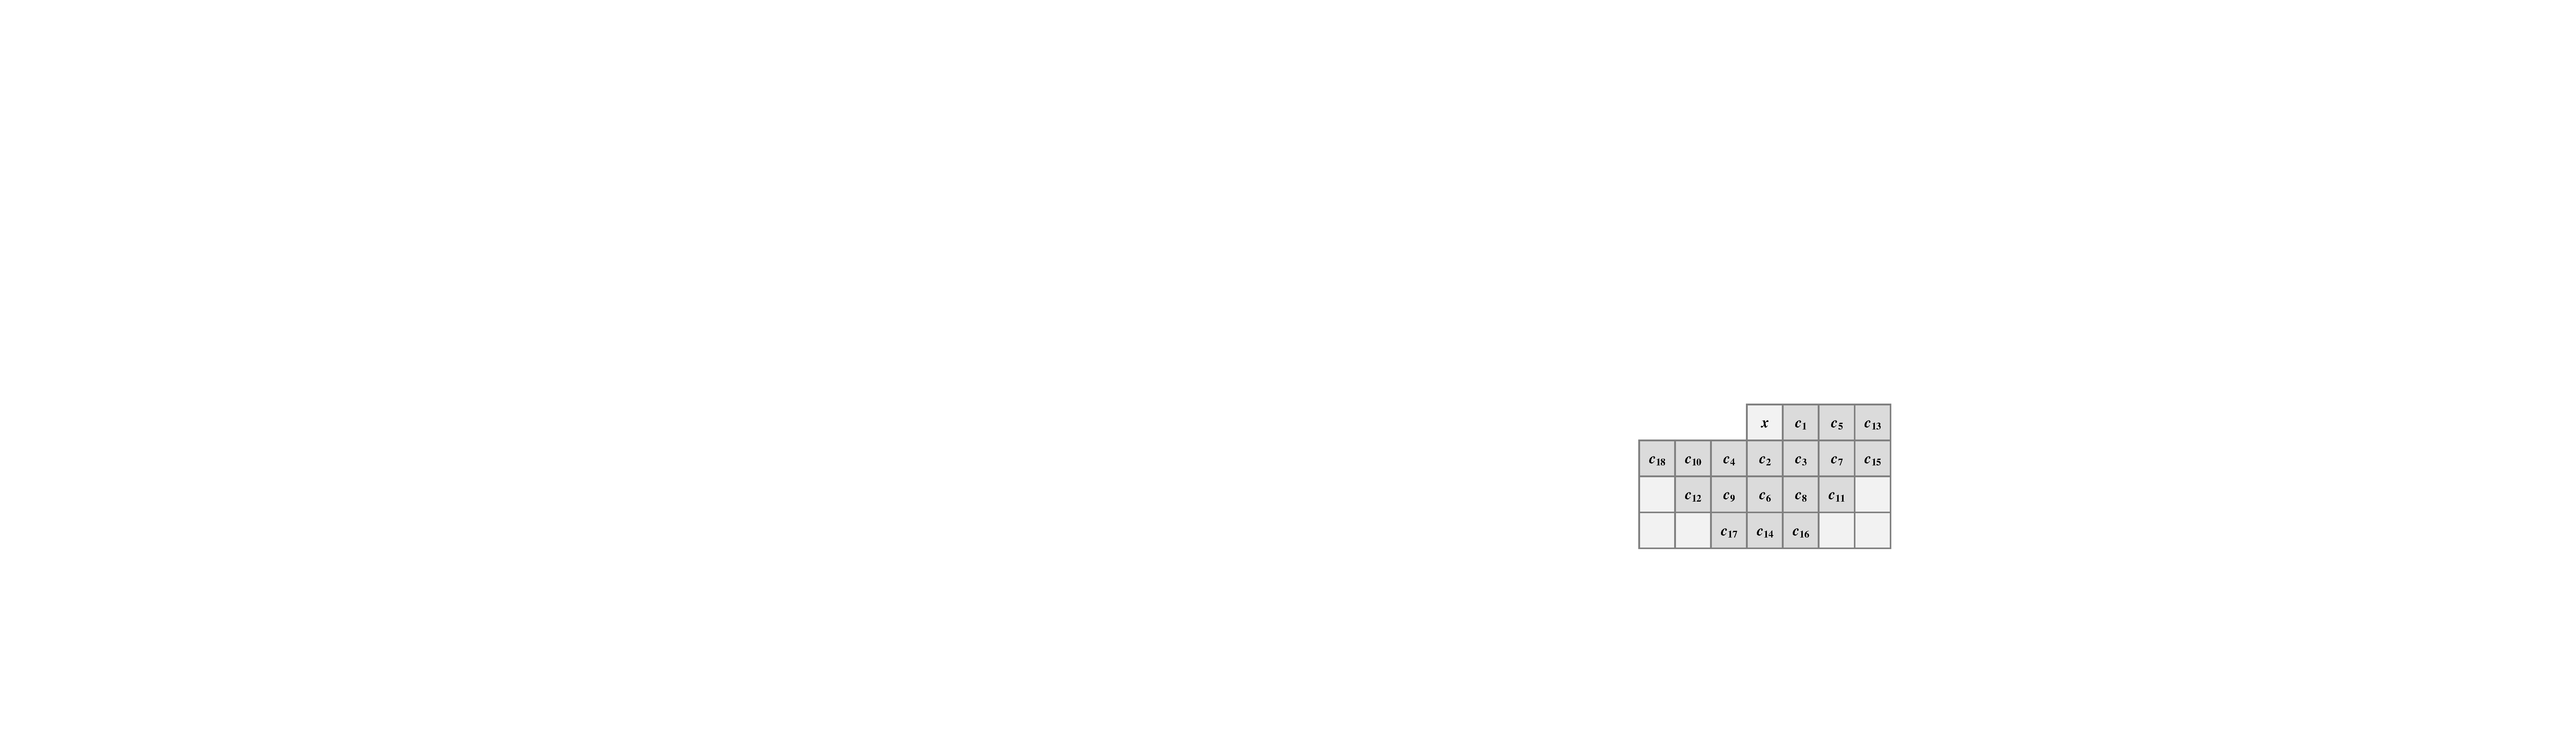
\includegraphics[width=1\textwidth]{figures/C4.pdf}
    \end{minipage}
}
\subfigure[$C_4$ of $n = 24$]{
    \begin{minipage}[t]{0.218\linewidth}
    \centering
    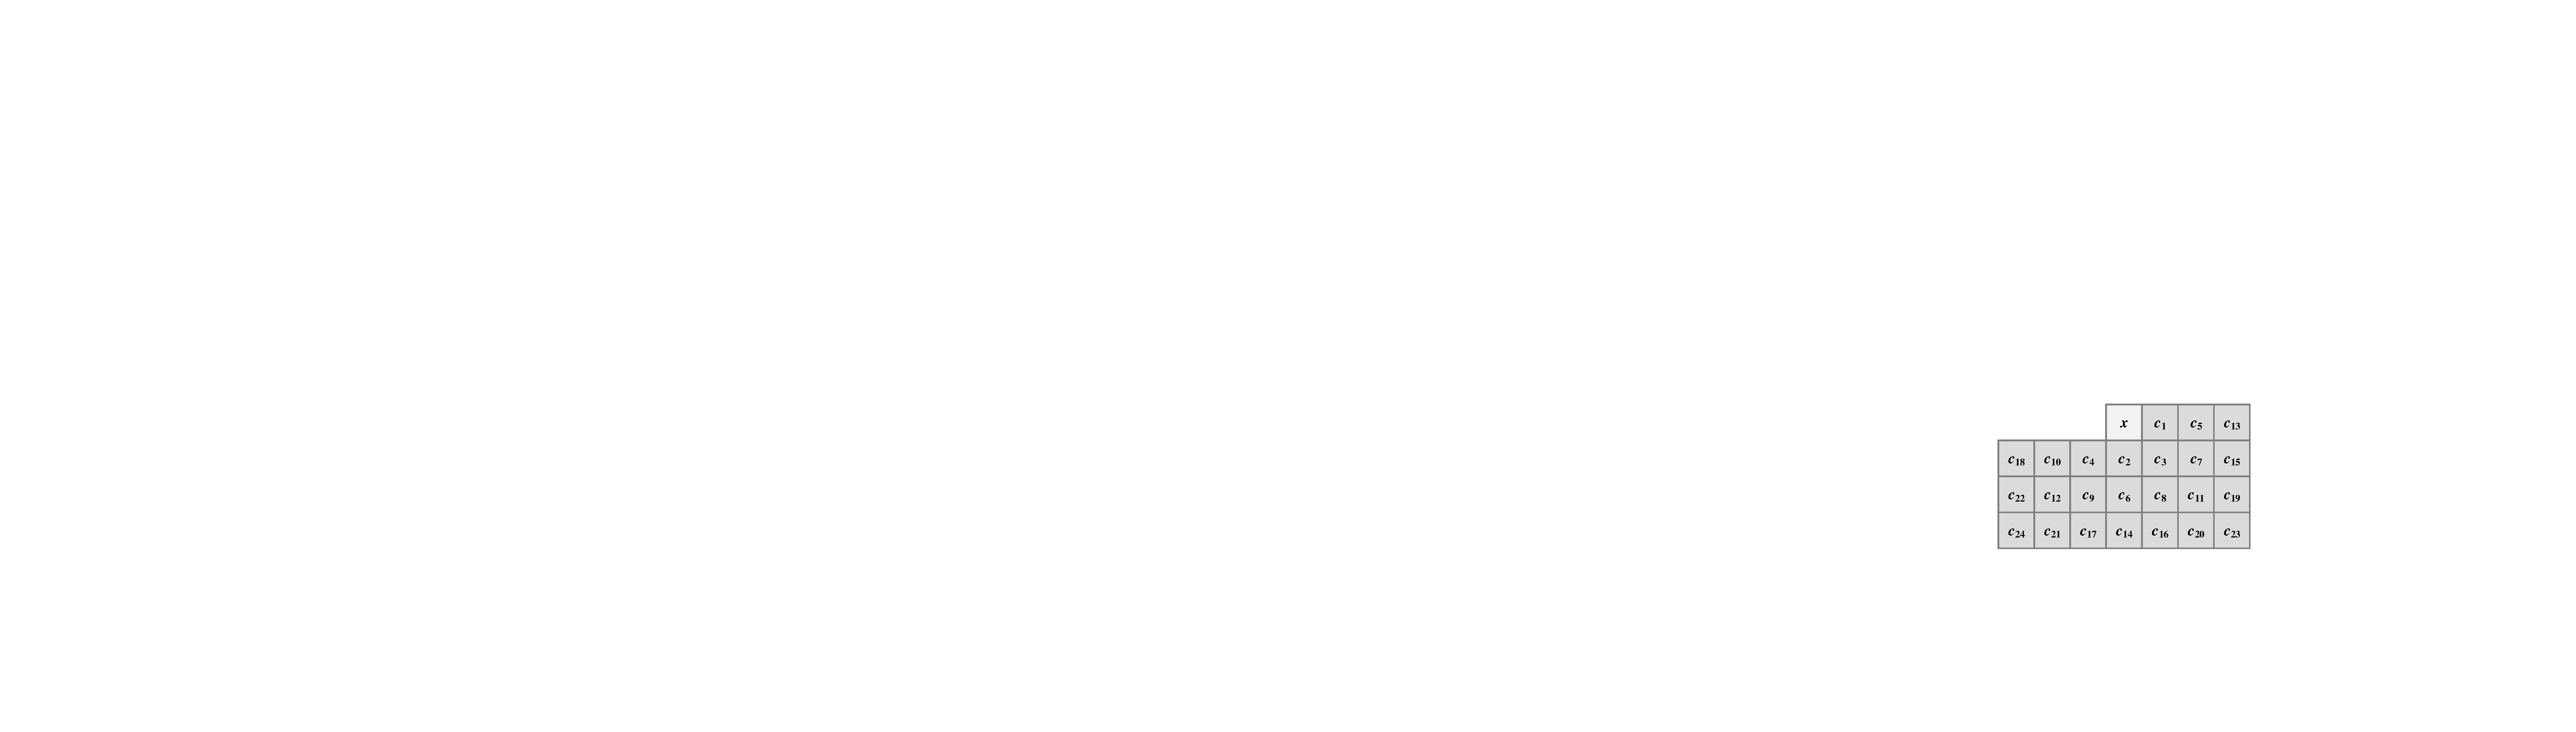
\includegraphics[width=1\textwidth]{figures/C3.pdf}
    \end{minipage}
}
\centering
\caption{Context pixels of $x$ by Extended PPVO.}
\label{Fig.Context3}
\end{figure*}

In Fig. \ref{Fig.Eval}, as an example, we focus on the two size context regions of $C_1$ and $C_2$. According to the curves, there are a few observations as follows.
\begin{enumerate}
  \item In Fig. \ref{Fig.Eval}(a), the maximum embedding capacity of $C_1$ is much larger than $C_2$. This is because almost pixels in the cover image with small $n$ is used for prediction while part of the pixels are skipped with larger size $C_2$.
  \item In Fig. \ref{Fig.Eval}(a), capacity increases very fast with the increase of threshold $T$ from a small value, especially curve of $C_1$. This indicates that pixels at smooth region are predicted accurate and are more suitable to be predicted.
  \item In Fig. \ref{Fig.Eval}(b), with the same threshold $T$, although the capacity of $C_2$ is smaller than $C_1$, proportion of shifted pixels of $C_2$ is much smaller than $C_1$. This observation illustrates that among the skipped pixels of $C_2$, the proportion of pixels that are predicted to be inaccurate is increase, which is no benefit to the performance.
\end{enumerate}
Through the above description, it shows that prediction with context pixels in smaller size context region achieves a large embedding capacity, but distortion also increases due to the pixels to be predicted inaccurately. And for the pixels in larger size context region, lots of inaccurately predicted pixels are skipped and proportion of sifted pixels is much less than the smaller size. But the embedding capacity is limited. Based on these consideration, a strategy of the multi-size based embedding method is given to combine the advantages of both size context.

In the proposed method, pixels on the cover images are divided into three parts by two thresholds $t_1$ and $t_2$ ($0 \leq t_1 \leq t_2$). Specifically, we let $X_{T} = \{x |\ {\rm NL}(x) < T\}$, which indicates the set of pixels with local complexity less than $T$. The region of pixels in $X_{t_1}$ are considered to be smooth, and these pixels are predicted by the context pixels of $C_1$. And the region of pixels in $X_{t_2} \setminus X_{t_1}$ are seem to be normal smooth, which are predicted by the context pixels of $C_2$. Other pixels are all skipped and do not participate in the embedding procedure. The above strategy is reasonable. In Fig. \ref{Fig.Eval}(b), it shows that the distance between the two curves is growing with the increase of threshold. This verify that in the area with higher complexity, more inaccurately predicted pixels are skipped with context pixels in $C_2$. Therefore, the pixels in smooth regions $X_{t_1}$ is predicted by the context pixels of $C_1$. This provides much more embedding capacity. And for the pixels in the normal regions $X_{t_2} \setminus X_{t_1}$, context pixels of $C_2$ are chosen as context pixels to predict, making the distortion as low as possible.

For example, Fig. \ref{Fig.EmbedExample} shows the the embedding procedures for the three types of pixels, where $(t_1, t_2) = (15, 25)$. For the first pixel value $x = 150$, because the complexity ${\rm NL} = 10$ of the pixel less than the small threshold $t_1$, the pixel is in a smooth region and context pixels $C = \{148, 150, 150, 148\}$ are chosen. The prediction-error of the pixel value is $p = 0$. One bit secret data $b = 1$ can be embedded by increasing the $x$ by $1$ to $\hat{x} = 151$. However, if context pixels of $C_2$ are chosen for prediction, the pixel wound be skipped because of $\min(C) < x < \max(C)$. For the second pixel $x = 135$, it is in normal region, where the complexity value ${\rm NL} = 24$ larger than $t_1$ but less than $t_2$. The context pixels $C = \{137, 136, 139, 138, 140, 135, 142, 137, 136, 139\}$ are chosen and prediction-error is $p = 0$. One bit data $b = 0$ can be embedded by remaining the pixel value $\hat{x} = x = 135$. If context pixels of $C_1$ are chosen, the prediction-error wound be $p = 1$ and no one bit data wound be embedded. The third pixel $x = 147$ is in a rough region whose complexity ${\rm NL} = 34$ larger than $t_2$ and it is skipped.
And for the purpose of finding suitable thresholds, let ${\rm H}_{t_1, t_2}$ as the histogram of prediction-errors derived from the pixels in $X_{t_1}$ with $C_1$ and pixels in $X_{t_2} \setminus X_{t_2}$ with $C_2$. For a given embedding capacity $EC$, the optimal thresholds $(t_1^*, t_2^*)$ are obtained by
\begin{equation}\label{eq:thresholds}
\begin{array}{ll}
\mathop{\arg\min}\limits_{0 \leq t_1 \leq t_2} & \frac{\frac{1}{2}{\rm H}_{t_1, t_2}(0) + \sum_{i \geq 1}{\rm H}_{t_1, t_2}(i)}{{\rm H}_{t_1, t_2}(0)}\\
s.t.                                    & {\rm H}_{t_1, t_2}(0) \geq EC
\end{array}.
\end{equation}
Fig. \ref{Fig.Thresholds} shows the optimal thresholds $(t_1^*, t_2^*)$ by (\ref{eq:thresholds}) for some capacities. It is note that the two optimal thresholds are positively correlated. However, it is difficult to find the exact relationship between them. So, in the optimization process, we find the optimal parameters by traversing all the values.
Fig. \ref{Fig.Eval0} shows three capacity-proportion curves, including two curves $C_1$ in blue and $C_2$ in red with a given context region, and a curve in pink $C_{12}$ that combines two different size context regions by the proposed method. Obviously, the proposed method achieve an less proportion of shifted pixels than others, which may lead to less embedding distortion.

\begin{figure*}
\centering
\subfigure[]{
    \begin{minipage}[t]{0.45\linewidth}
    \centering
    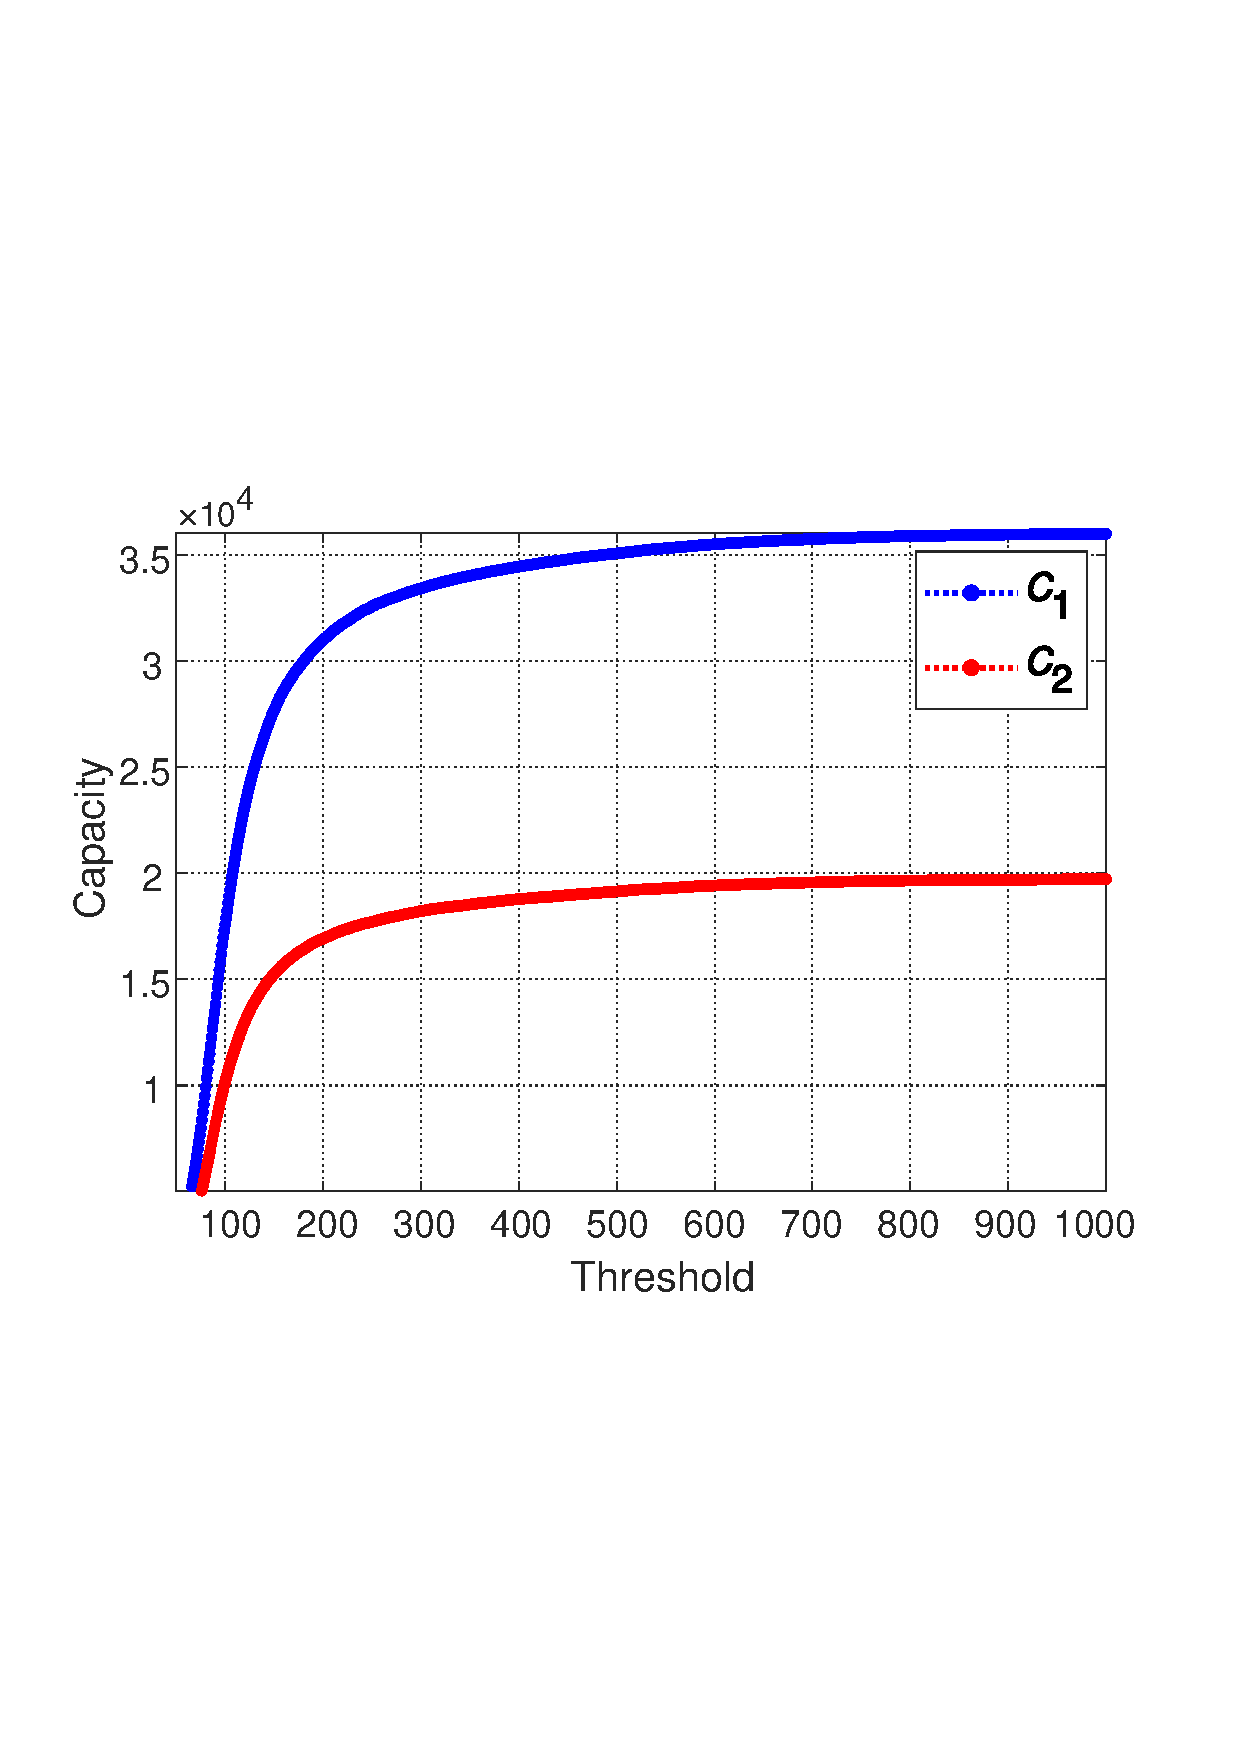
\includegraphics[width=1\textwidth]{figures/CapLena.pdf}
    \end{minipage}
}
\qquad
\subfigure[]{
    \begin{minipage}[t]{0.46\linewidth}
    \centering
    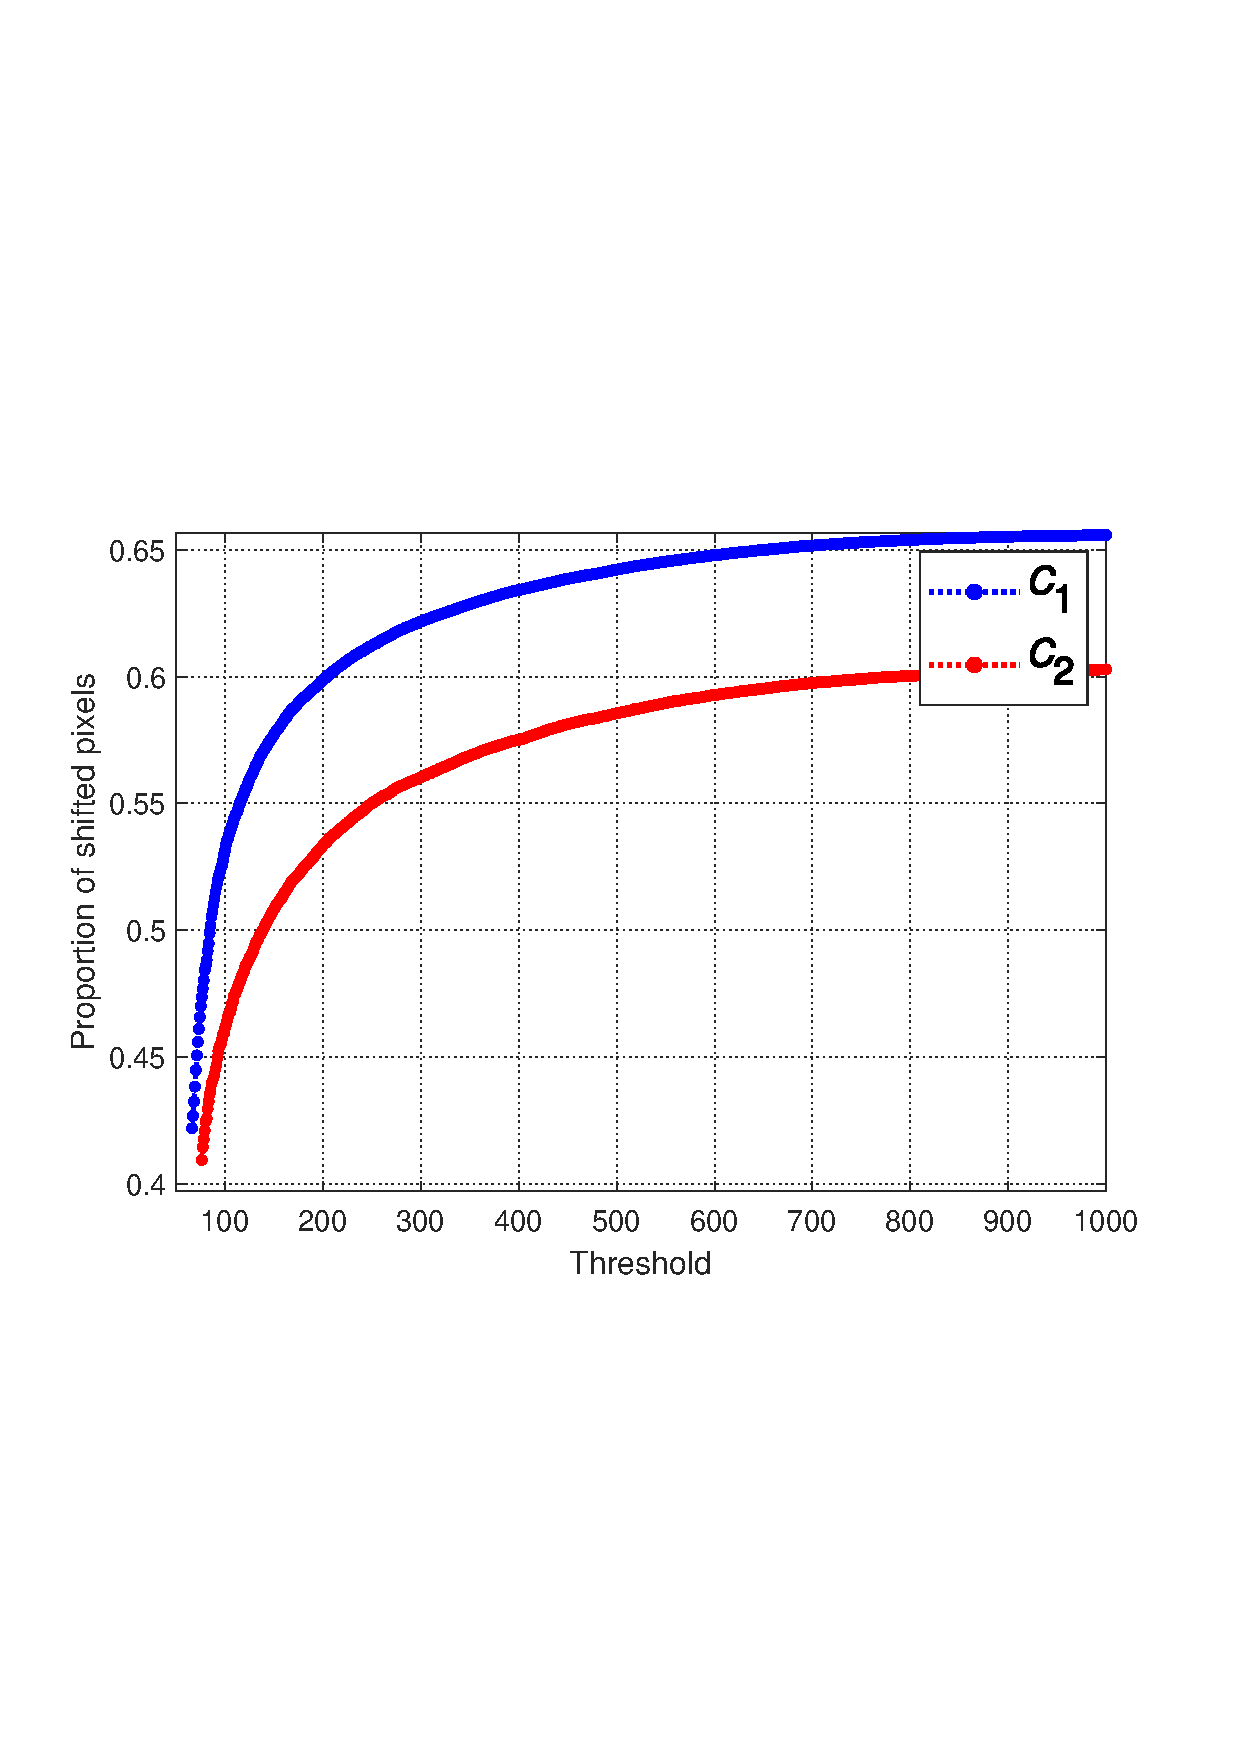
\includegraphics[width=1\textwidth]{figures/thPropLena.pdf}
    \end{minipage}
}
\centering
\caption{Eval of Lena.}
\label{Fig.Eval}
\end{figure*}
\begin{figure*}
\centering
    \begin{minipage}[t]{0.5\linewidth}
    \centering
    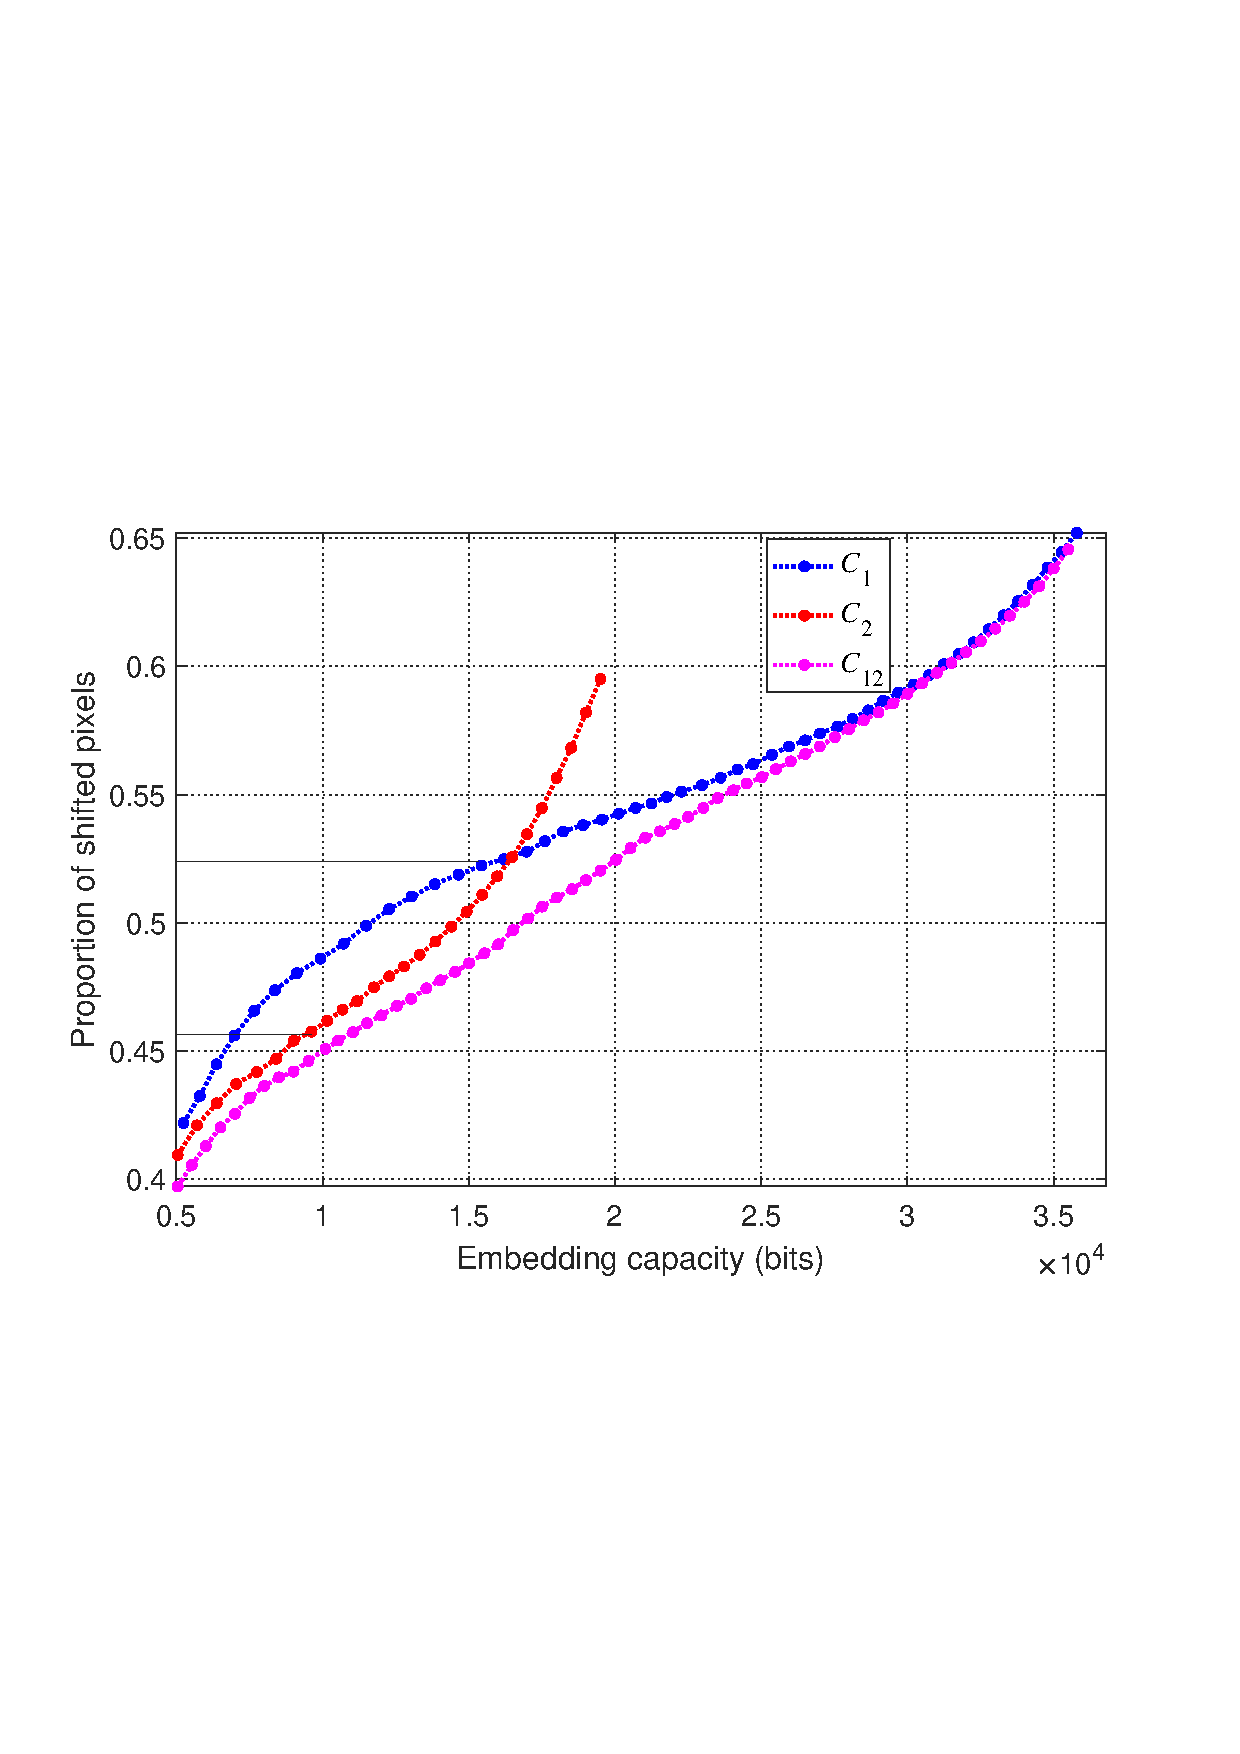
\includegraphics[width=1\textwidth]{figures/PropLenaNoT.pdf}
    \end{minipage}
\centering
\caption{Eval of Lena.}
\label{Fig.Eval0}
\end{figure*}

\begin{figure*}
\centering
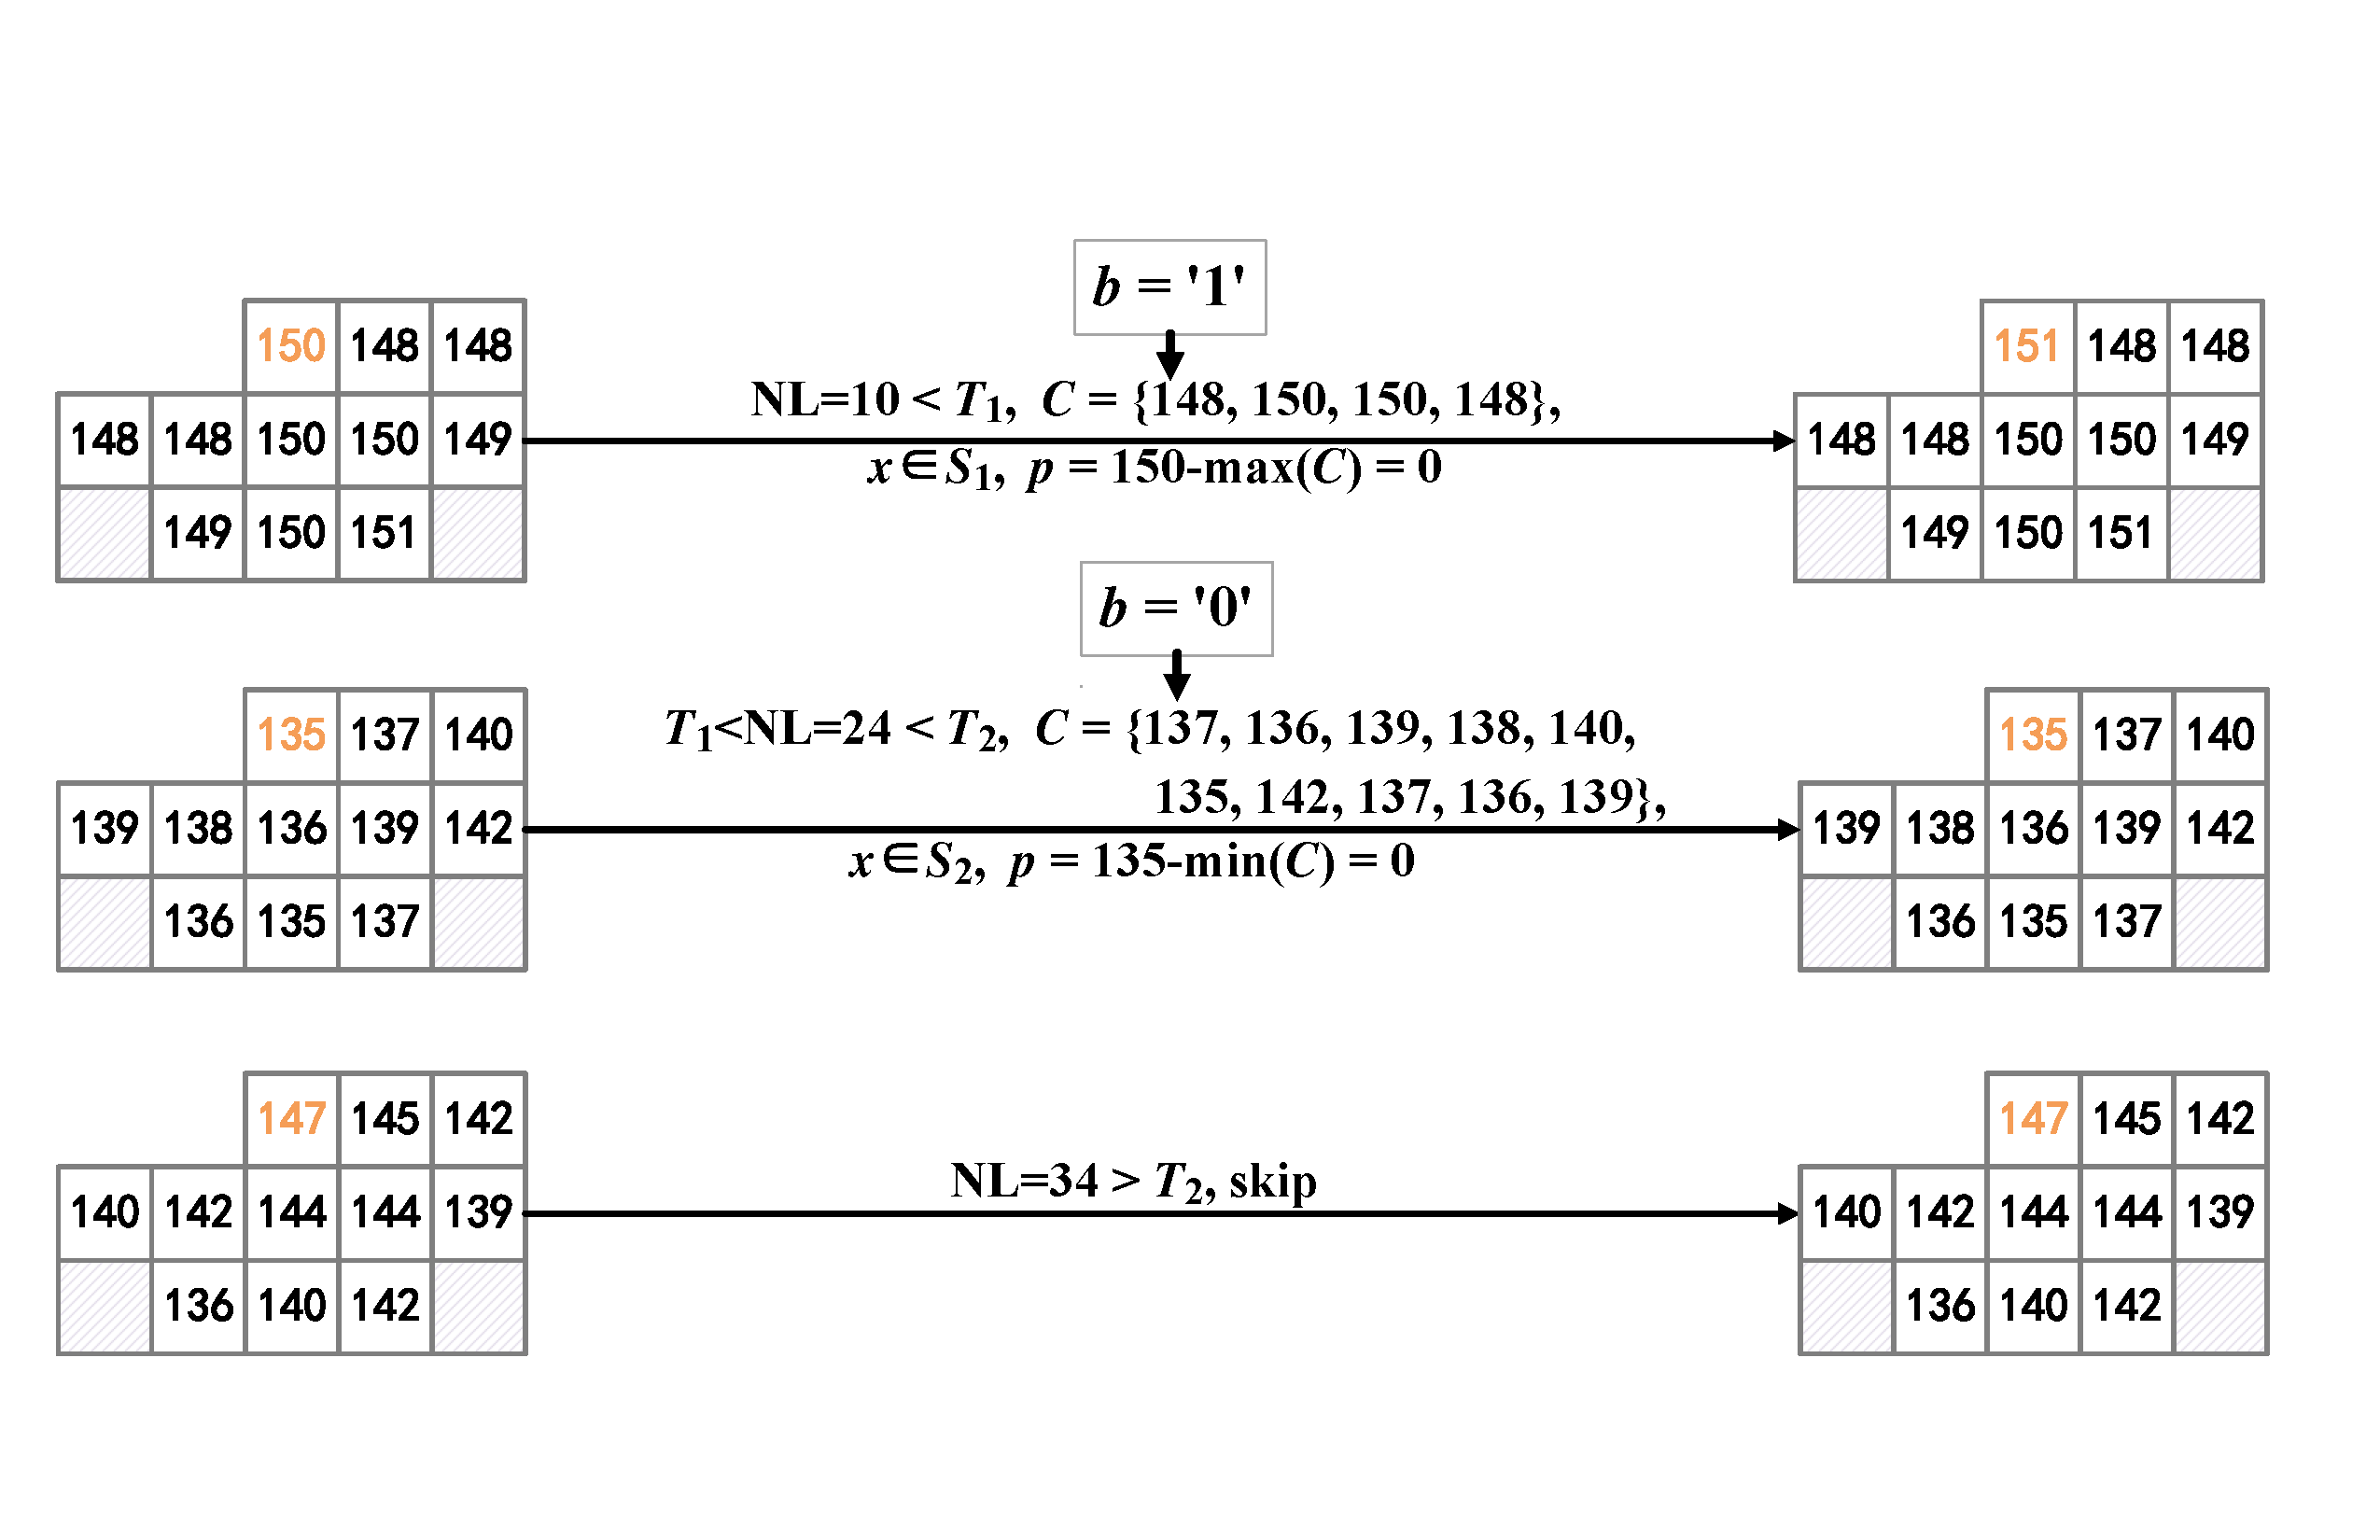
\includegraphics[width=0.7\textwidth]{figures/EmbedwithTh.pdf}
\centering
\caption{Example.}
\label{Fig.EmbedExample}
\end{figure*}

\begin{figure*}
\centering
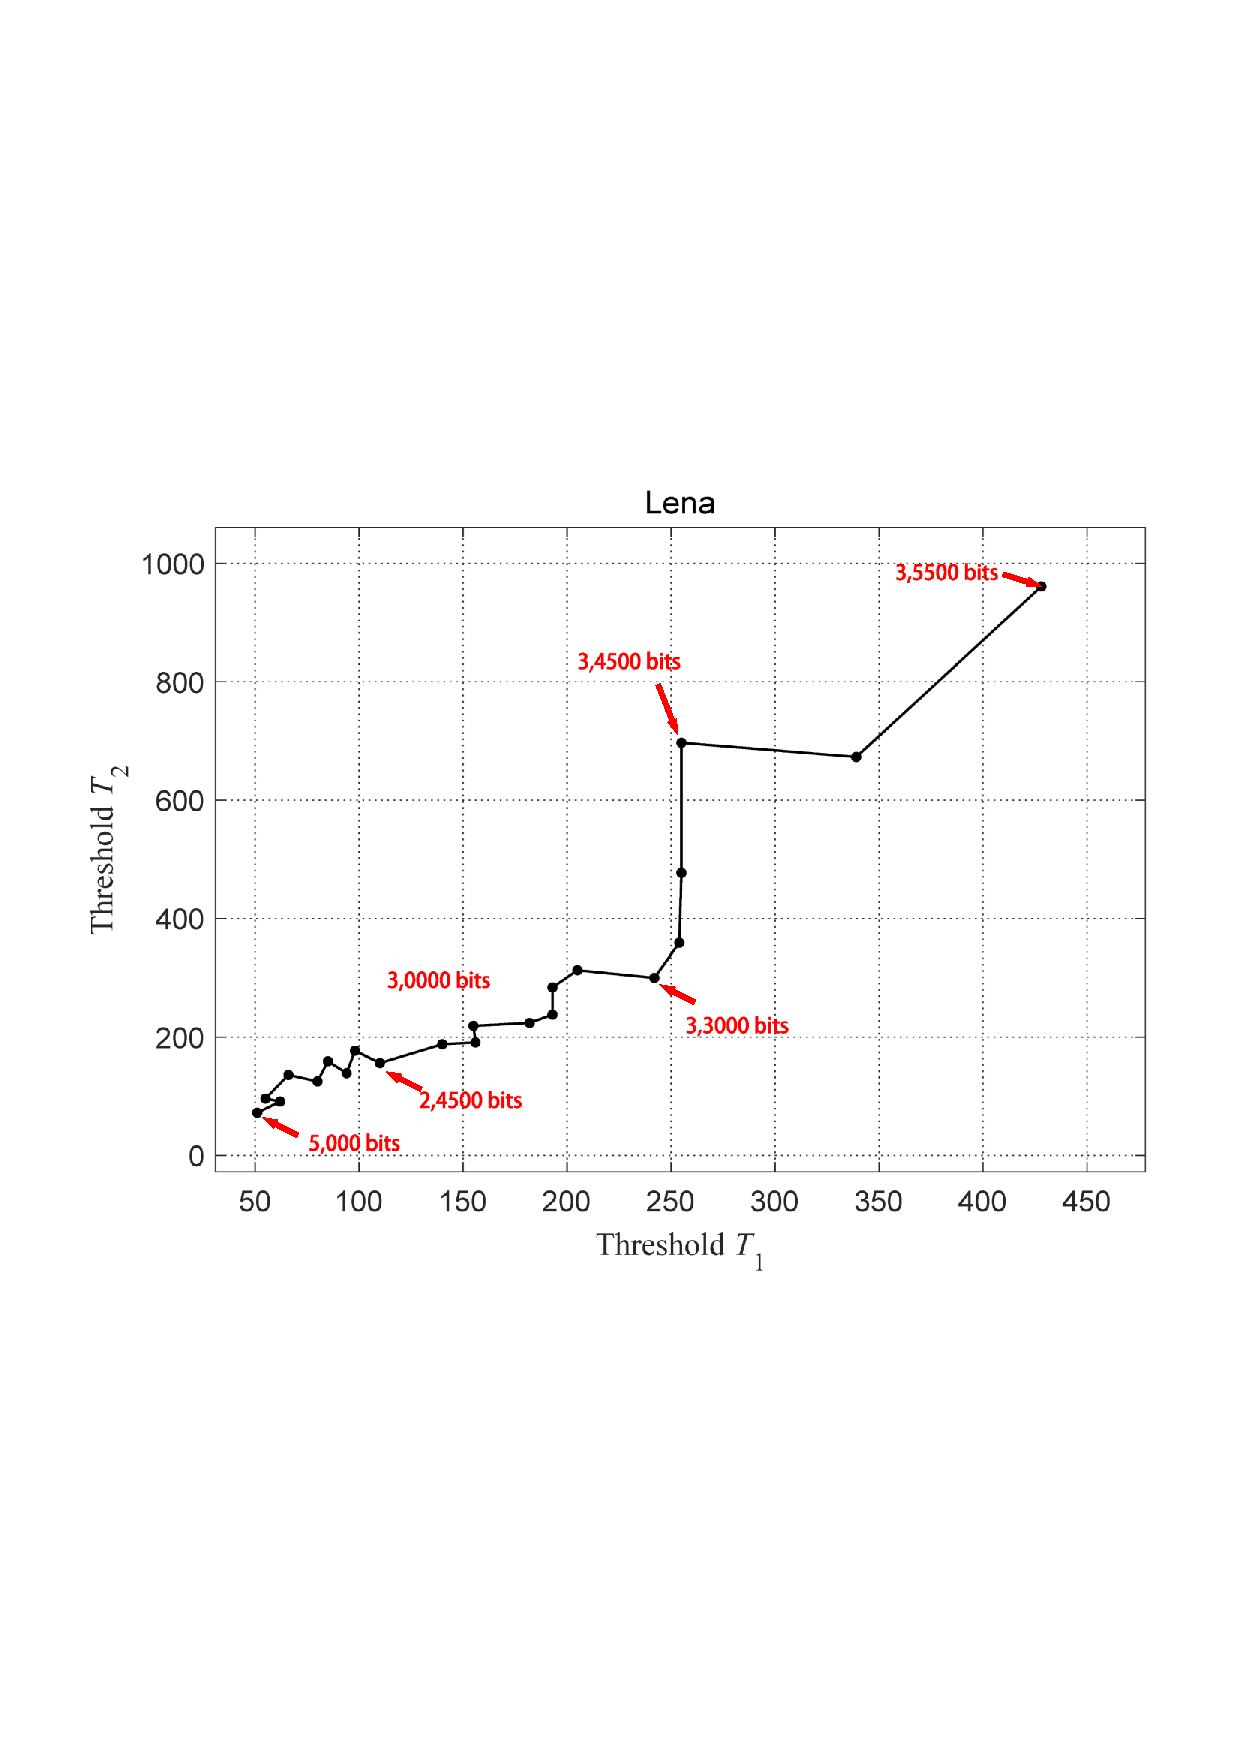
\includegraphics[width=0.5\textwidth]{figures/Thresholds.pdf}
\centering
\caption{Thresholds.}
\label{Fig.Thresholds}
\end{figure*}

In addition, more context sizes can be considered to combine to further decrease the proportion. We set $N$ as the number of context regions to be considered. As shown in Fig. \ref{fig:size}, for each given capacity, $N$ is from $1$ to $4$, corresponding the sizes $C_1 \in \{C_1\}$, $C_{12} \in \{C_1, C_2\}$, $C_{123} \in \{C_1, C_2, C_3\}$ and $C_{1234} \in \{C_1, C_2, C_3, C_4\}$, respectively. It shows that although the embedding performance increases with the increase of $N$, it is already very small when $N = 4$. Therefore, balancing the embedding performance and embedding time complexity, we set $N = 3$ as a suitable size number. Therefore,  for the current pixel, there are three complexity thresholds $\{t_1, t_2, t_3\}$ to choose context pixels The smoother the area where the pixel is, the less context pixels are used to predict.

\begin{figure*}
\centering
\subfigure{
\begin{minipage}[t]{0.4\linewidth}
\centering
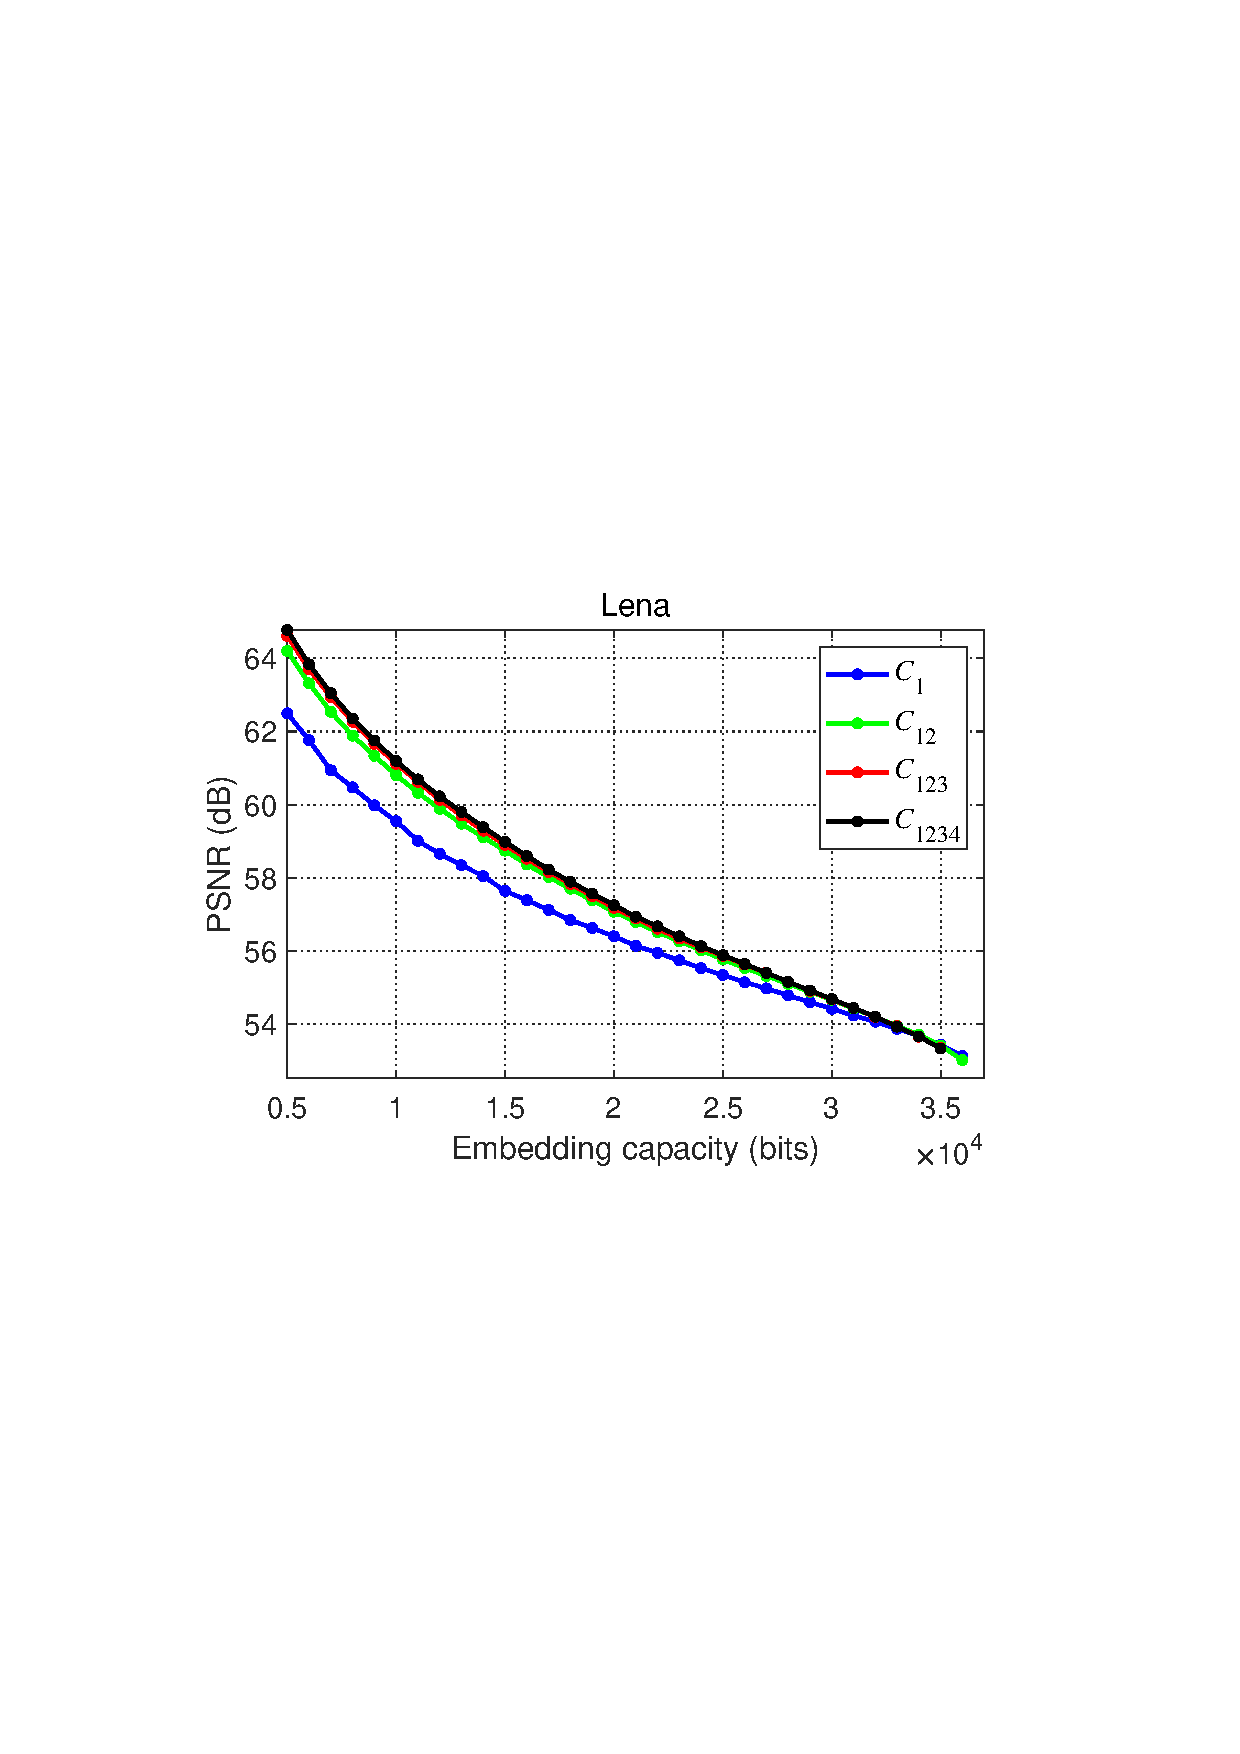
\includegraphics[width=1\textwidth]{figures/Result/size/Lena.pdf}
\end{minipage}
}
\qquad
\subfigure{
\begin{minipage}[t]{0.412\linewidth}
\centering
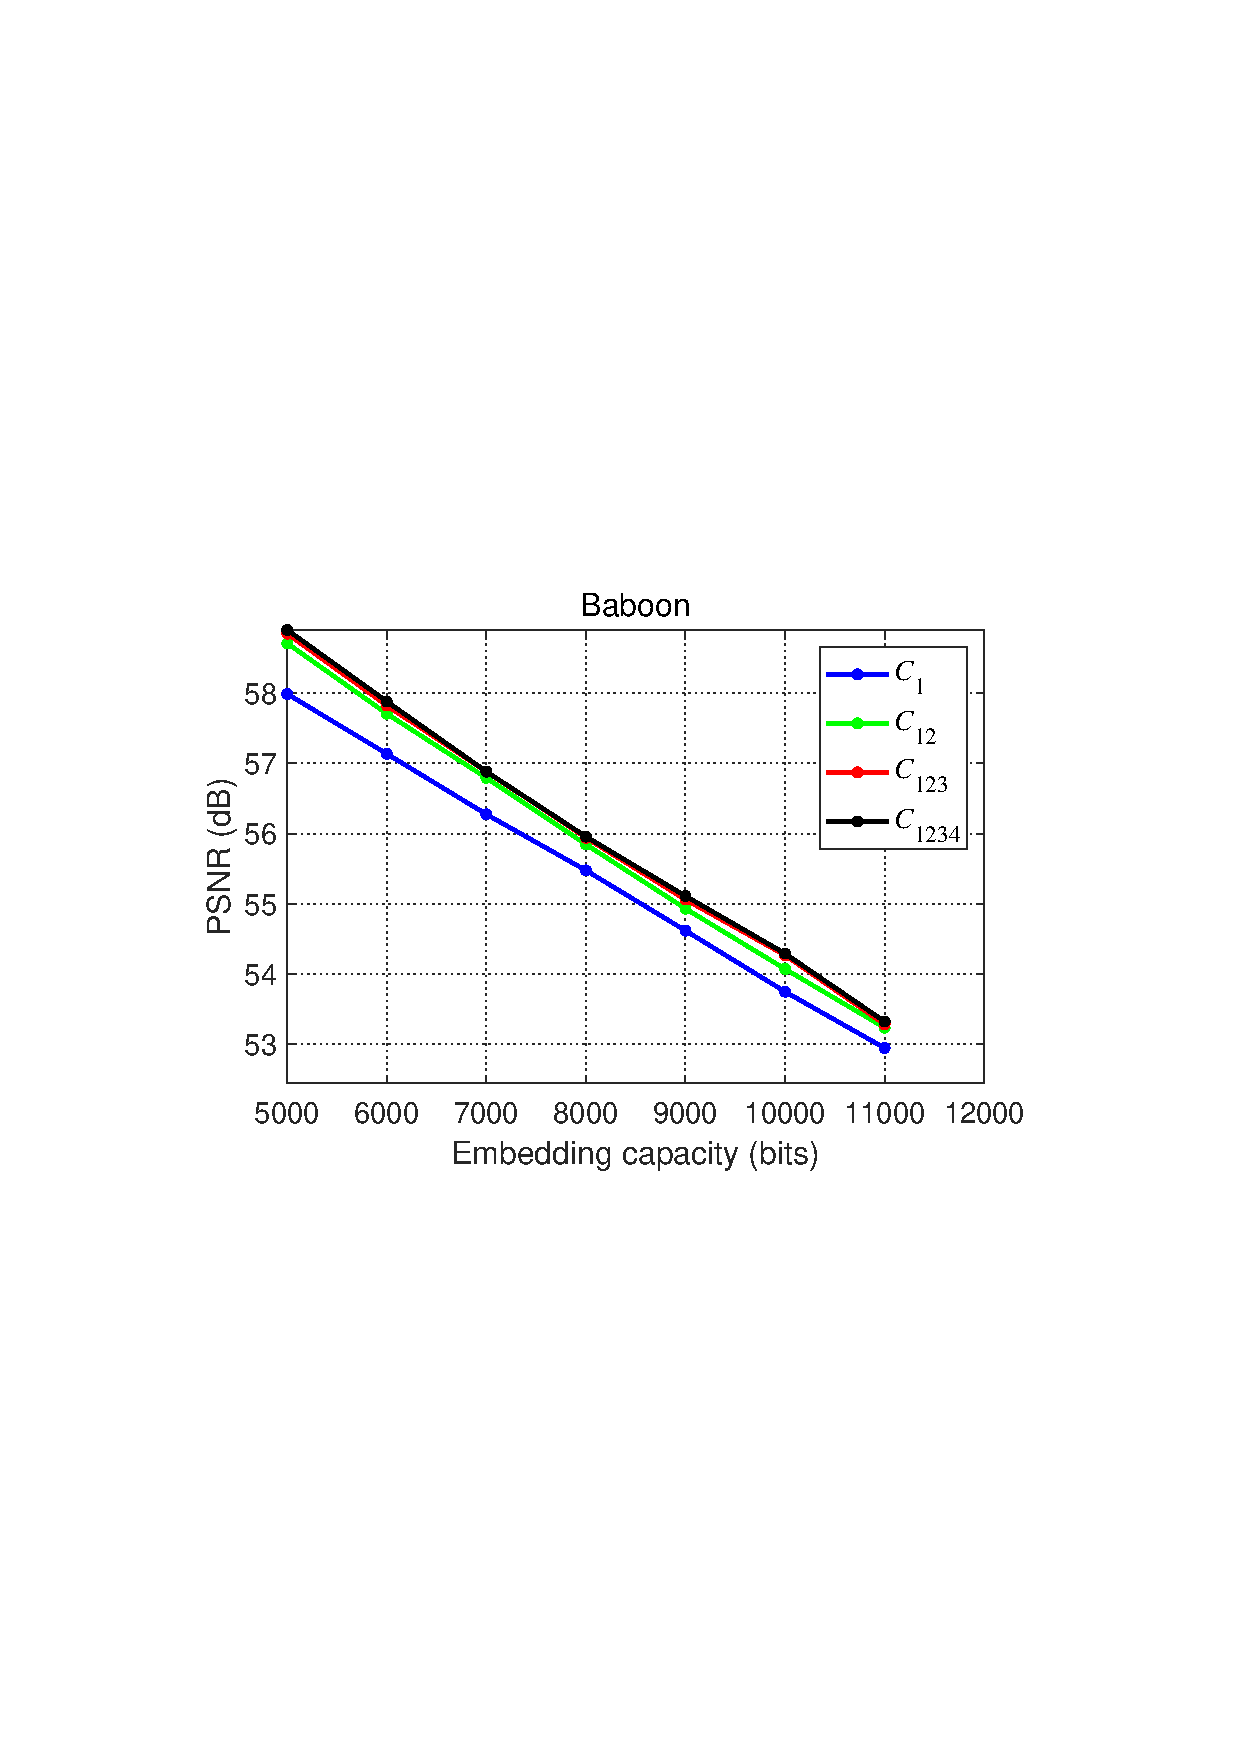
\includegraphics[width=1\textwidth]{figures/Result/size/Baboon.pdf}
\end{minipage}
}
\centering
\caption{size.}
\label{fig:size}       % Give a unique label
\end{figure*}


\subsection{Data Embedding and Extraction Procedures}\label{sec:3.3}
The data embedding procedure is divided into the following steps to introduce as follow. Firstly, a location map ${\rm LM}$ is constructed to solve overflow/underflow problem. For $i$-th pixel $x_i$, if $x_i = 0$ or $x_i = 255$, we assign ${\rm LM}(i) = 1$. Otherwise, we assign ${\rm LM}(i) = 0$. All pixels equals $255$ are modified to $254$ and $0$ are modified to $1$. Because ${\rm LM}$ records all the locations where the overflow/underflow may occur, original pixels can be recovered. Next, for the given several context sizes $\{C_1, C_2, C_3\}$, the complexity ${\rm NL}(i)$ of current pixel value $x_i$ is calculated the sum of the absolution differences of the horizontal and vertical of every two adjacent pixels belong to the largest size context $C_3$. And context pixels to predict $x_i$ are selected by comparing ${\rm NL}(i)$ with the given thresholds $\{t_1, t_2, t_3\}$($0 \leq T_1 < T_2 < T_3$ ), which is similar to the procedure described in section \ref{sec:3.2}. Then, $x_i$ is predicted by the chosen context pixels yo derive the prediction-error $e$ by (\ref{eq:PE}) and one bit data is embedded by modifying $x_i$ to $\tilde{x}_i$ by (\ref{eq:PPVOMPixel}). The steps of prediction and embedding are performed pixel-by-pixel until all secret data is embedded and current pixel position is recorded as $k_{\rm end}$. Finally, for reversibility, some auxiliary information should be used for blind decoding such as
\begin{itemize}
  \item the complexity thresholds $t_1$, $t_2$ and $t_3$ ($11 \times 3 = 33$ bits),
  \item the pixel position where data embedding ends $k_{\rm end}$ (18 bits),
  \item length of compressed location map $L$ (18 bits),
  \item the compressed location map ${\rm LM}$ ($L$ bits).
\end{itemize}
To embed the auxiliary information, LSB of first $69 + L$ bits pixels of the image is recorded to obtain a binary vector $V_{\rm LSB}$ and then replaced by the auxiliary information. $V_{\rm LSB}$ is embedded into pixels after $x_{k_{\rm end}}$ by the same way as secret data embedding. During the whole embedding procedure, the threshold $t_1$ is selected from 1 and increased by 1 iteratively and $j$-th threshold $t_j$ is selected from $t_{j-1} + 1$ and increased by 1 iteratively. The optimal thresholds are obtained by traversing all values of pixel complexities.

The extraction procedure is an opposite process. Firstly, auxiliary information is gotten by reading LSB of first $69 + L$ bits pixels and replaced by LSB of pixels after $x_{k_{\rm end}}$. Next, for marked pixel value $\tilde{x}$, complexity is computed as the same as embedding procedure by extracting data pixel-by-pixel in reverse order. And, with extracted three complexity thresholds $\{t_1, t_2, t_3\}$, the same context pixels $C$ of $\tilde{x}$ as original pixel value $x$ can be obtained. Then, prediction-error $\tilde{e}$ of the marked pixel value $\tilde{x}$ is computed by (\ref{eq:dPE}). And the original pixel value $x$ is recovered by (\ref{eq:dPPVOMPE}). Meanwhile, the secret data $b$ can be extracted that $b = 1$ if $\tilde{e} \in \{-1, 1\}$ or $b = 0$ if $\tilde{e} = 0$. Finally, original image is recovered by ${\rm LM}$ referring the embedding procedure.

%----------------------------------------------------------------------------------------
\section{Experimental Results}\label{sec:4}
% N \in {1, 2, 3, 4}, N=4 been chosen,
In this section, experimental results of proposed method are presented. The performance is compared with three typical PVO-based methods of Peng \emph{et al.} \cite{Peng2014IPVO}, Ou \emph{et al.} \cite{Ou2014PVOk} and Qu \emph{et al.} \cite{Qu2015PPVO}. The proposed method is implemented on MatLab version 2018a on a tower server (SUPERMICRO LT-7038AX) and for a given embedding capacity, embedding procedure can be implemented less than four seconds.

The experimental results are evaluated on eight standard gray-scale $512 \times 512$-sized images including Lena, Baboon, Airplane, Barabra, Lake, Boat, Peppers and Eliane. Fig. \ref{fig:size} shows the performance comparison on the eight test images. The capacity increases from 5,000 bits to the largest embedding capacity with a step of 1,000 bits. The figures reveal that the proposed method is superior to other three PVO-basd methods. Specifically, the performance comparison for given capacities of 10,000 bits and 20,000 bits are represented in Table~\ref{tab:10000bits} and Table~\ref{tab:20000bits}. Besides, the optimal parameters $(t_1^*, t_2^*, t_3^*)$ of proposed method are also listed in the tables. It can be seen that the optimal thresholds are different on different test images and differen embedding capacities. Thus, considering that the computational complexity is not high, exhaustively all threshold combinations are feasible.

The improved PVO-based RDH proposed by Peng \emph{et al.} \cite{Peng2014IPVO} is an improvement of the original PVO RDH \cite{Li2013PVO}. The cover image is first divided into non-overlapping and equal size sub-blocks, and then secret data is embedding into the prediction-errors of largest/smallest value pixels in each sub-block. Compared with the original PVO-based RDH, in the improved PVO-based RDH, the smooth blocks are utilized for data embedding by considering the original order of pixels in each block. Fig. \ref{fig:size} shows that its performance is mediocre compared with other methods. Through Table~\ref{tab:10000bits} and Table~\ref{tab:20000bits}, the proposed method obtain an improvement of PSNR of 0.90 dB and 0.99 dB respectively. The PVO-$k$ proposed by Qu \emph{et al.} \cite{Qu2015PPVO} is another improvement of the original PVO RDH which aims to make full use of smooth blocks as well. In this method, the blocks with more than one largest/smallest pixel value are utilized by modifying the largest/smallest pixel values concurrent. It shows a better performance than the improved PVO-based method but it is still unsatisfactory. According to Table~\ref{tab:10000bits} and Table~\ref{tab:20000bits}, the proposed method obtain an improvement of PSNR of 0.63 dB and 0.78 dB respectively.

The PPVO-based RDH proposed by Qu \emph{et al.} \cite{Qu2015PPVO} is different from traditional PVO-based RDH methods. It breaks through the block constraint and prediction process is implemented pixel by pixel. In this method, the embedding procedure is implemented for fifteen times with different number of context pixels from 1 to 15, and number of the best performance is chosen as the final parameter. It means that, whatever the pixel is in a smooth or complex area, the context pixels for prediction is constant. The performance of PPVO achieve a superior performance than traditional PVO-based RDH methods. According to the Table~\ref{tab:10000bits} and Table~\ref{tab:20000bits}, the proposed method considers the impact of the number of context pixels and get a increase of PSNR of 0.57 dB and 0.44 dB respectively.

%For PPVO, 15 times of embedding are performed under each embedding capacity in every image to find a proper number of context pixels from 1 to 15, and the results with highest PSNR are shown in Fig. 11. This method changes the block-by-block manner used in PVO and IPVO to pixel-by-pixel manner to predict each pixel and improves the performance by using more pixels in smooth area than IPVO. However, its performance can be further improved by a more accurate full-enclosing predictor as well as a variable bin used for extension in multiple PEHs. Specifically, the proposed methods outperforms PPVO in almost all the images except for the slight weakness in Elaine when EC is bigger than 17,000, and it improves PPVO by 0.74 dB for an embedding capacity of 10,000 bits and 0.65 dB for 20,000 bits in average according to Table 3 and Table 4.

\begin{figure*}
\centering
\subfigure{
\begin{minipage}[t]{0.415\linewidth}
\centering
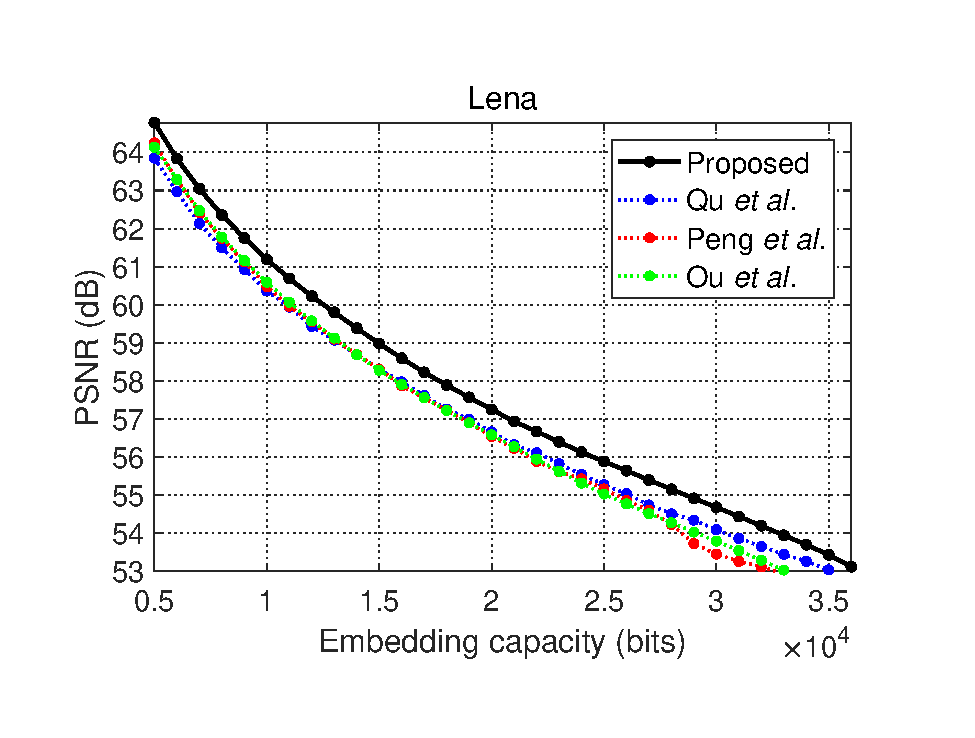
\includegraphics[width=1\textwidth]{figures/Result/capacity/Lena.pdf}
\end{minipage}
}
\subfigure{
\begin{minipage}[t]{0.43\linewidth}
\centering
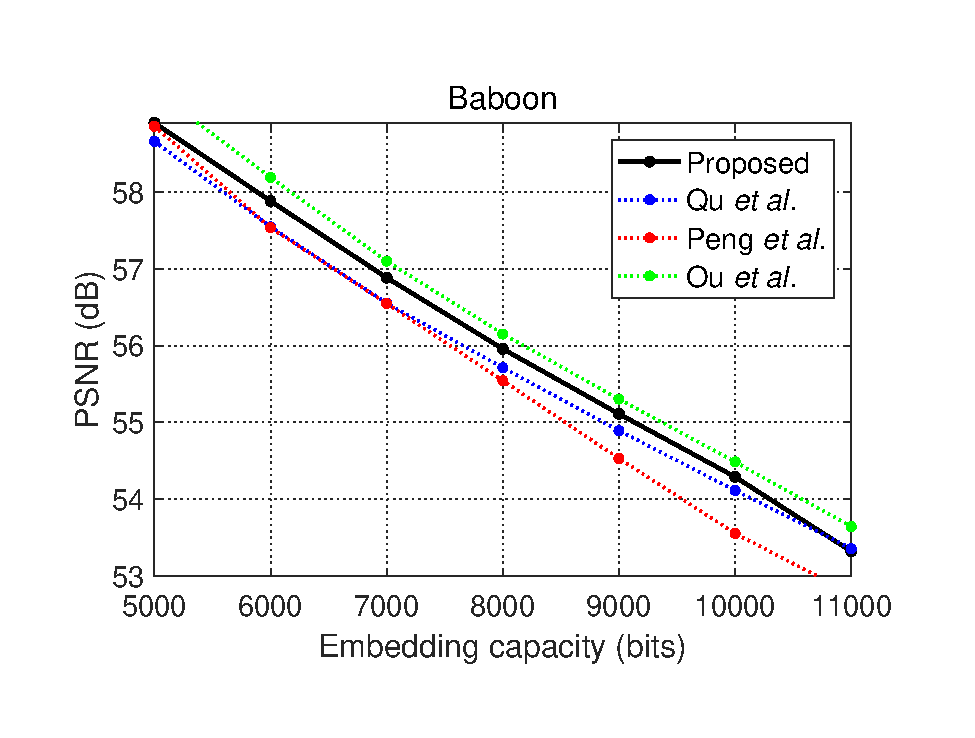
\includegraphics[width=1\textwidth]{figures/Result/capacity/Baboon.pdf}
\end{minipage}
}

\subfigure{
\begin{minipage}[t]{0.415\linewidth}
\centering
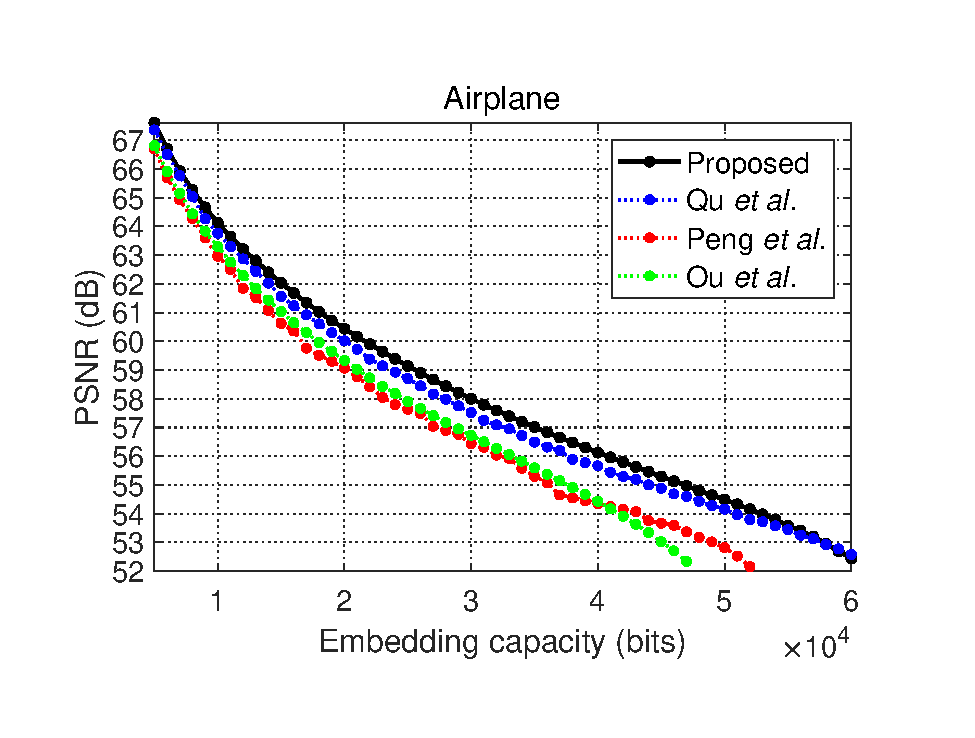
\includegraphics[width=1\textwidth]{figures/Result/capacity/Airplane.pdf}
\end{minipage}
}
\subfigure{
\begin{minipage}[t]{0.415\linewidth}
\centering
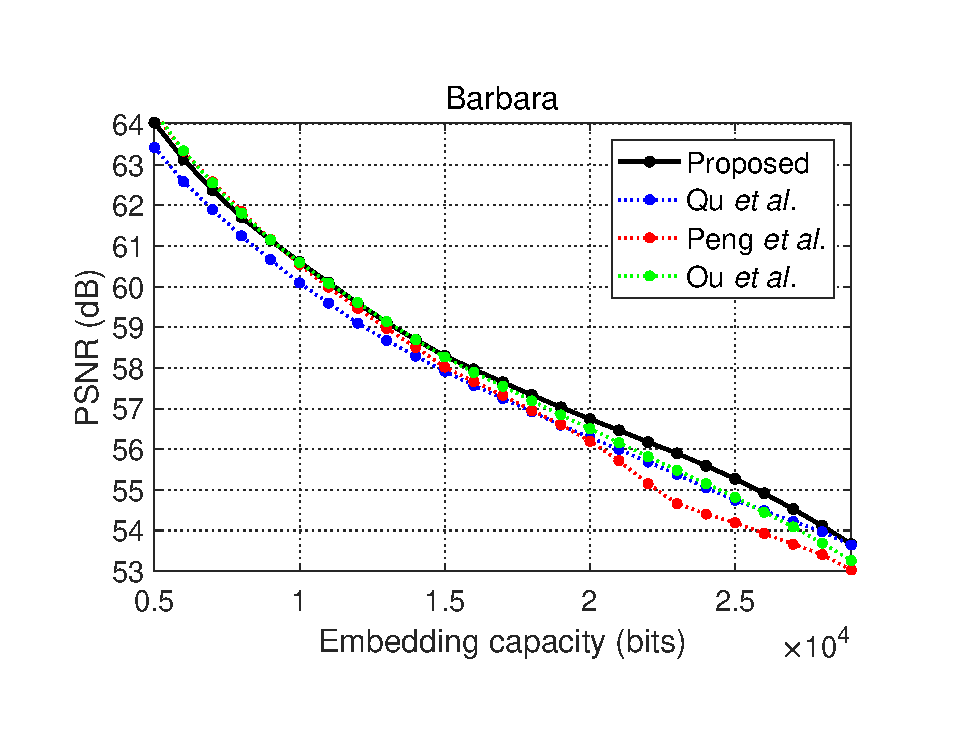
\includegraphics[width=1\textwidth]{figures/Result/capacity/Barbara.pdf}
\end{minipage}
}

\subfigure{
\begin{minipage}[t]{0.415\linewidth}
\centering
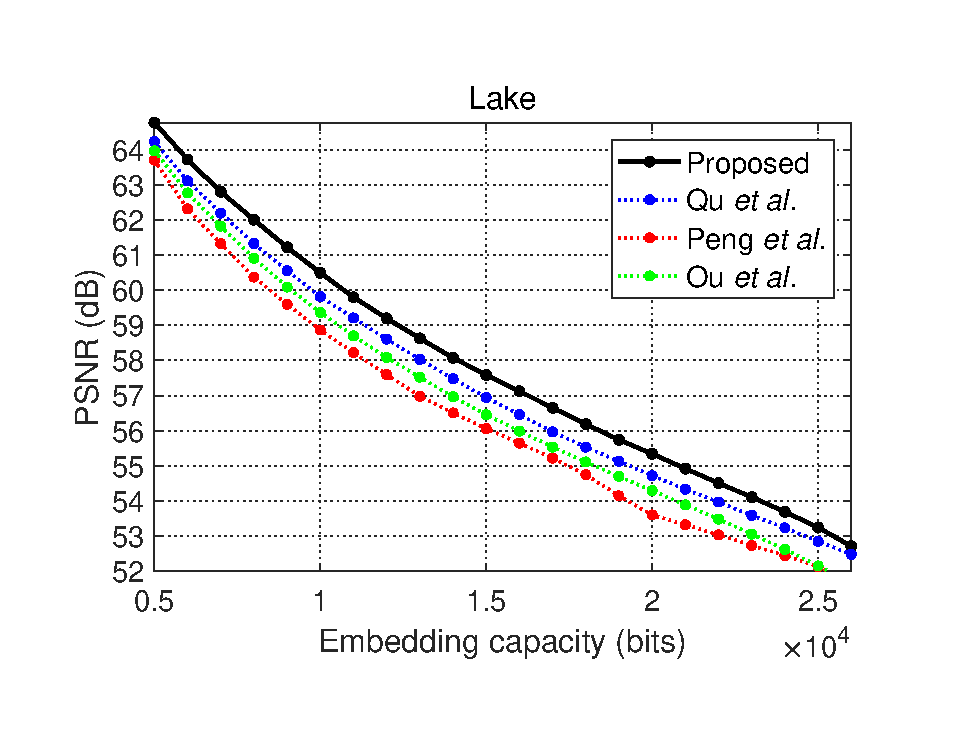
\includegraphics[width=1\textwidth]{figures/Result/capacity/Lake.pdf}
\end{minipage}
}
\subfigure{
\begin{minipage}[t]{0.42\linewidth}
\centering
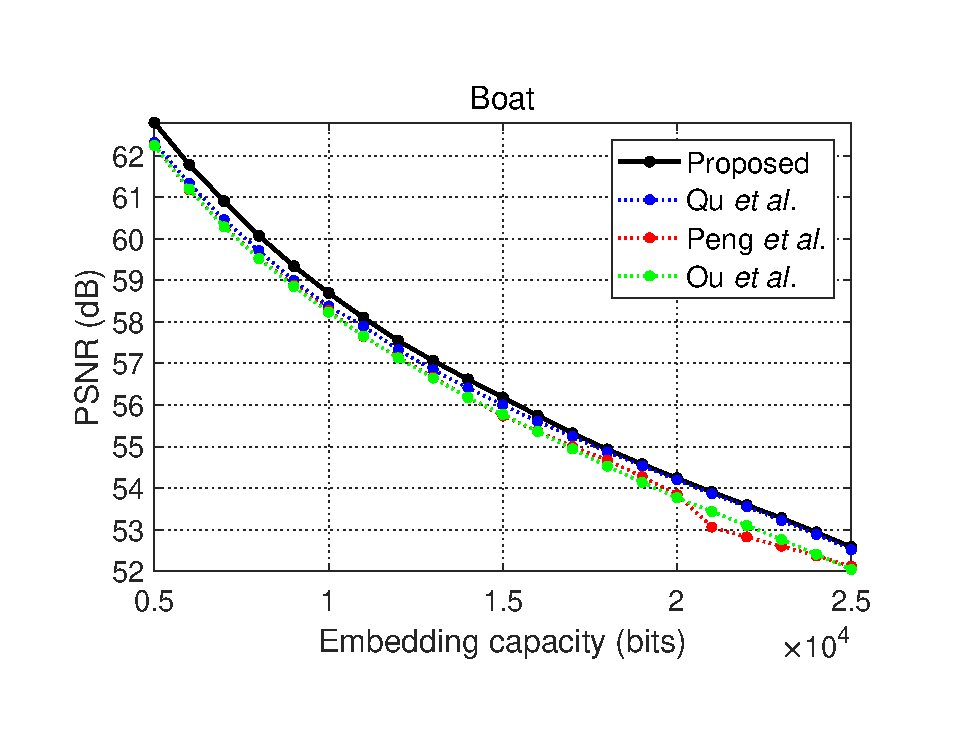
\includegraphics[width=1\textwidth]{figures/Result/capacity/Boat.pdf}
\end{minipage}
}

\subfigure{
\begin{minipage}[t]{0.415\linewidth}
\centering
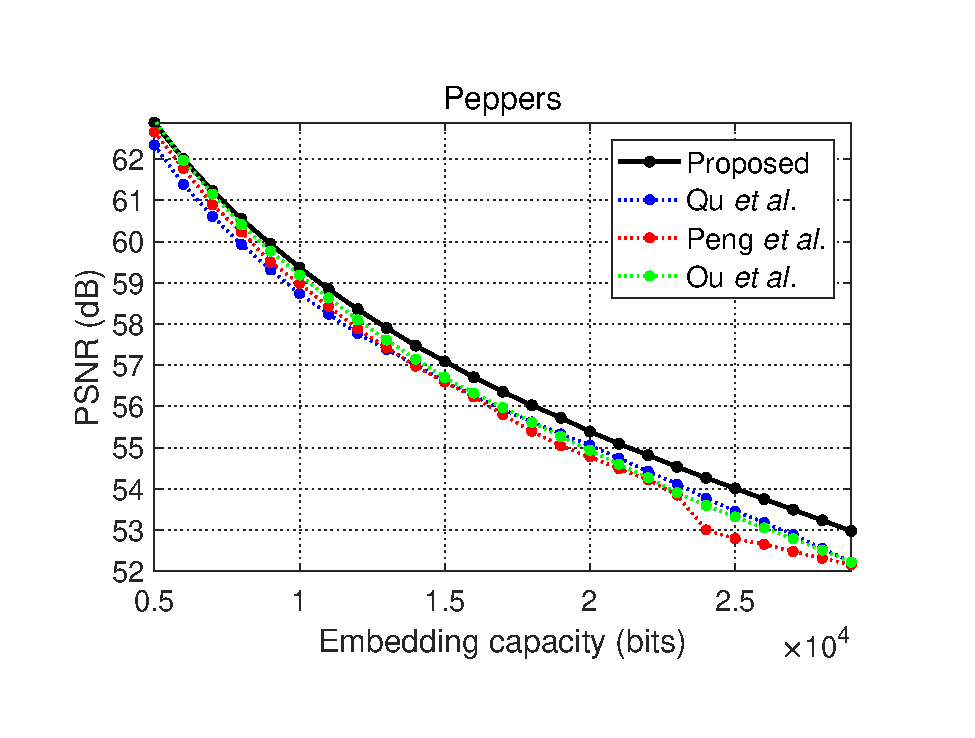
\includegraphics[width=1\textwidth]{figures/Result/capacity/Peppers.pdf}
\end{minipage}
}
\subfigure{
\begin{minipage}[t]{0.415\linewidth}
\centering
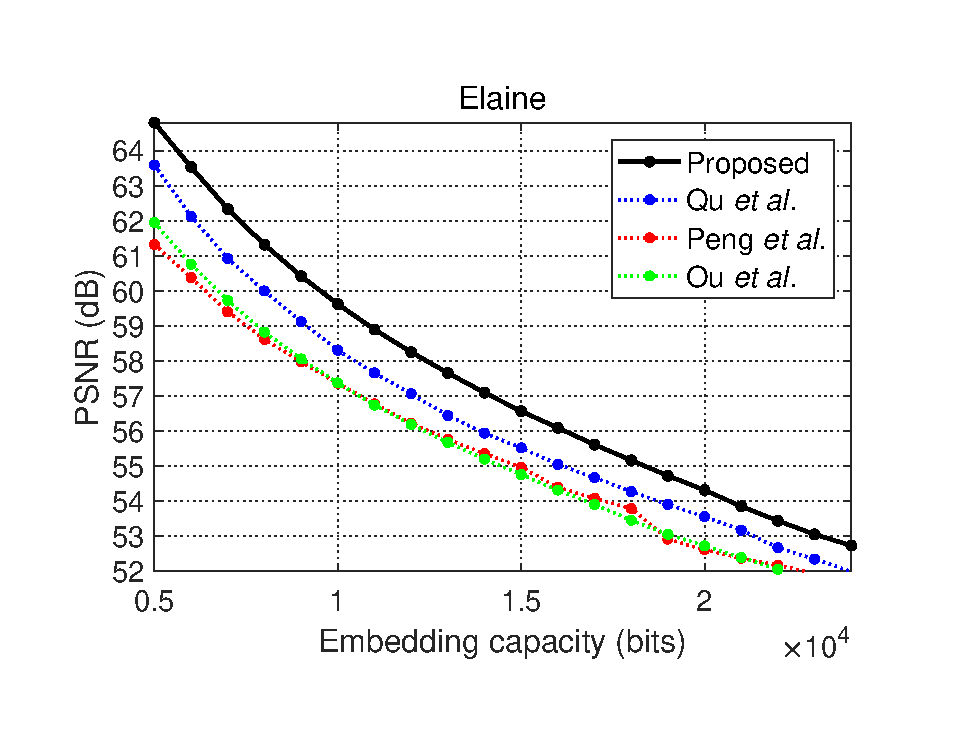
\includegraphics[width=1\textwidth]{figures/Result/capacity/Elaine.pdf}
\end{minipage}
}
\centering
\caption{capacity.}
\label{fig:capacity}       % Give a unique label
\end{figure*}

\begin{table*}
\scriptsize
\centering
\caption{Comparison of PSNR (dB) among the proposed method and the PVO-based methods of Peng \emph{et al.} \cite{Peng2014IPVO}, Ou \emph{et al.} \cite{Ou2014PVOk} and Qu \emph{et al.} \cite{Qu2015PPVO}. The embedding capacity is 10,000 bits. The optimal parameters of the proposed method are also listed.}
\setlength{\tabcolsep}{3mm}{
\begin{tabular}{lccccc}
\hline
%\toprule
\multirow{2}{*}{Images}             &
\multirow{2}{*}{Peng \emph{et al.}} &
\multirow{2}{*}{Ou \emph{et al.}}   &
\multirow{2}{*}{Qu \emph{et al.}}   &
\multicolumn{2}{c}{Proposed Method}\\
%\cmidrule(r){1} \cmidrule(r){2} \cmidrule(r){3} \cmidrule(r){4} \cmidrule(r){5-6}
\cline{5-6}
                        &                    &                       &                   & PSNR &           $(t_1^*, t_2^*, t_3^*)$   \\
%\midrule
\hline
Lena                    & 60.49                 & 60.59             & 60.36              & \textbf{61.12}   & (39,45,73)        \\ % (52,102,129)
Baboon                  & 53.58                 & 54.48             & 54.11              & \textbf{54.27}   & (337,465,1099)    \\ % 0.01
Airplane                & 62.97                 & 63.29             & 63.76              & \textbf{64.06}   & (16,17,22)        \\ % (22,31,32)
Barbara                 & 60.48                 & 60.59             & 60.08              & \textbf{60.59}   & (17,66,79)        \\ % (75,94,121)
Lake                    & 58.81                 & 59.36             & 59.81              & \textbf{60.50}   & (54,83,112)       \\ % (156,193,227)
Boat                    & 58.26                 & 58.23             & 58.37              & \textbf{58.70}   & (78,96,144)       \\ % (159,191,266)
Peppers                 & 58.97                 & 59.18             & 58.73              & \textbf{59.32}   & (29,92,121)       \\ % (96,196,186)
Elaine                  & 57.37                 & 57.37             & 58.30              & \textbf{59.46}   & (82,116,142)      \\ % (165,334,452)
\hline
Average                 & 58.86                 & 59.13             & 59.19              & \textbf{59.76}   &                   \\
\hline
\end{tabular}
}
\label{tab:10000bits}
\end{table*}

\begin{table*}
\scriptsize
\centering
\caption{Comparison of PSNR (dB) among the proposed method and the PVO-based methods of Peng \emph{et al.} \cite{Peng2014IPVO}, Ou \emph{et al.} \cite{Ou2014PVOk} and Qu \emph{et al.} \cite{Qu2015PPVO}. The embedding capacity is 20,000 bits. The optimal parameters of the proposed method are also listed.}
\setlength{\tabcolsep}{3mm}{
\begin{tabular}{lccccc}
%\toprule
\hline
\multirow{2}{*}{Images}             &
\multirow{2}{*}{Peng \emph{et al.}} &
\multirow{2}{*}{Ou \emph{et al.}}   &
\multirow{2}{*}{Qu \emph{et al.}}   &
\multicolumn{2}{c}{Proposed Method}\\
%\cmidrule(r){1} \cmidrule(r){2} \cmidrule(r){3} \cmidrule(r){4} \cmidrule(r){5-6}
\cline{5-6}
                        &                    &                       &                   & PSNR &           $(t_1^*, t_2^*, t_3^*)$   \\
\hline
Lena                    & 56.56                 & 56.58             & 56.65              & \textbf{57.18}   & (52,102,129)      \\
Airplane                & 59.07                 & 59.33             & 60.01              & \textbf{60.40}   & (22,31,32)        \\
Barbara                 & 56.20                 & 56.50             & 56.28              & \textbf{56.74}   & (75,94,121)       \\
Lake                    & 53.53                 & 54.29             & 54.71              & \textbf{55.34}   & (156,193,227)     \\
Boat                    & 53.83                 & 53.76             & 54.19              & \textbf{54.24}   & (159,191,266)     \\
Peppers                 & 54.77                 & 54.93             & 55.05              & \textbf{55.39}   & (96,196,186)      \\
Elaine                  & 52.65                 & 52.71             & 53.55              & \textbf{54.21}   & (165,334,452)     \\
\hline
Average                 & 55.23                 & 55.44             & 55.78              & \textbf{56.22}\\
\hline
\end{tabular}
}
\label{tab:20000bits}
\end{table*}

%\begin{table}
%\centering
%\caption{Comparison of PSNR (dB) among the proposed method and the PVO-based methods of Peng \emph{et al.} \cite{Peng2014IPVO}, Ou \emph{et al.} \cite{Ou2014PVOk} and Qu \emph{et al.} \cite{Qu2015PPVO}. The embedding capacity is 10,000 bits.}
%\setlength{\tabcolsep}{3mm}{
%\begin{tabular}{lccccc}
%\hline
%{Images}                & Qu \emph{et al.}   & Peng \emph{et al.}    & Ou \emph{et al.}  & Proposed\\
%\hline
%Lena                    & 60.36              & 60.49                 & 60.59             & \textbf{61.12}\\ % 0.01
%Baboon                  & 54.11              & 53.58                 & 54.48             & \textbf{54.27}\\ % 0.01
%Airplane                & 63.76              & 62.97                 & 63.29             & \textbf{64.06}\\ % 0.01
%Barbara                 & 60.08              & 60.48                 & 60.59             & \textbf{60.59}\\ % 0.01
%Lake                    & 59.81              & 58.81                 & 59.36             & \textbf{60.50}\\ % 0.03
%Boat                    & 58.37              & 58.26                 & 58.23             & \textbf{58.70}\\ % 0.01
%Peppers                 & 58.73              & 58.97                 & 59.18             & \textbf{59.32}\\ % 0.01
%Elaine                  & 58.30              & 57.37                 & 57.37             & \textbf{59.46}\\ % 0.02
%\hline
%Average                 & 59.19              & 58.86                 & 59.13             & \textbf{59.76}\\
%\hline
%\end{tabular}
%}
%\label{tab:10000bits}
%\end{table}

%\begin{table}
%\centering
%\caption{Comparison of PSNR (dB) among the proposed method and the PVO-based methods of Peng \emph{et al.} \cite{Peng2014IPVO}, Ou \emph{et al.} \cite{Ou2014PVOk} and Qu \emph{et al.} \cite{Qu2015PPVO}. The embedding capacity is 20,000 bits.}
%\setlength{\tabcolsep}{3mm}{
%\begin{tabular}{lccccc}
%\hline
%{Images}                & Qu \emph{et al.}   & Peng \emph{et al.}    & Ou \emph{et al.}  & Proposed\\
%\hline
%Lena                    & 56.65              & 56.56                 & 56.58             & \textbf{57.18}\\ % 0.01
%Airplane                & 60.01              & 59.07                 & 59.33             & \textbf{60.40}\\ % 0.01
%Barbara                 & 56.28              & 56.20                 & 56.50             & \textbf{56.74}\\ % 0.01
%Lake                    & 54.71              & 53.53                 & 54.29             & \textbf{55.34}\\ % 0.03
%Boat                    & 54.19              & 53.83                 & 53.76             & \textbf{54.24}\\ % 0.01
%Peppers                 & 55.05              & 54.77                 & 54.93             & \textbf{55.39}\\ % 0.01
%Elaine                  & 53.55              & 52.65                 & 52.71             & \textbf{54.21}\\ % 0.02
%\hline
%Average                 & 55.78              & 55.23                 & 55.44             & \textbf{56.22}\\
%\hline
%\end{tabular}
%}
%\label{tab:20000bits}
%\end{table}

%----------------------------------------------------------------------------------------
\section{Conclusion}\label{sec:5}
In this paper, based on an extended PPVO predictor and multi-size based embedding method, an extended PPVO-based RDH method is proposed. For each pixel to be predicted, surrounding pixels in left lower and right lower direction are utilized to derive a sharper PEH. And next, the relationship between context region size and local complexity is explored. The pixels in smooth area are predicted by context pixels in a small region size. And for the pixels in complex area, context pixels are chosen by a larger region size. The proposed method is verified that is more satisfactory than other several state-of-the-art PVO-based RDH methods.

%----------------------------------------------------------------------------------------
\section*{Acknowledgement}
This work was supported by the National Key Research and Development of China (No. 2016YF-B0800404), the National Science Foundation of China (Nos. 61572052 and U1736213), and the Fundamental Research Funds for the Central Universities (Nos. 2017RC008 and 2018JBZ001).

\bibliographystyle{elsarticle-num}

\bibliography{Cited}


\end{document}
